\documentclass[11pt]{report}


\usepackage[utf8]{inputenc}
\usepackage{geometry}
\usepackage{graphicx}
\graphicspath{ {figures/} }
\usepackage{amsmath}
\usepackage[colorlinks=true, linkcolor=blue, urlcolor=blue, citecolor=blue]{hyperref}
\usepackage{xcolor}
\usepackage{color}
\usepackage{listings}
\usepackage{xcolor}
\usepackage{titlesec}
\usepackage{nomencl}
\usepackage{lipsum}
\usepackage{setspace}
\usepackage{caption}
\usepackage{subcaption}
\usepackage{float}
\usepackage{framed}

\usepackage{cite}
\usepackage{times}
\usepackage{tabularx}
\definecolor{codeblue}{rgb}{0.1, 0.1, 0.8}
\definecolor{codegreen}{rgb}{0, 0.6, 0}
\definecolor{codegray}{rgb}{0.5, 0.5, 0.5}
\definecolor{codepurple}{rgb}{0.6, 0, 0.6}
\definecolor{backcolor}{rgb}{0.95, 0.95, 0.92}


\lstdefinestyle{mystyle}{
    backgroundcolor=\color{backcolor},   
    commentstyle=\color{codegreen},
    keywordstyle=\color{codeblue},
    numberstyle=\tiny\color{codeblue},
    stringstyle=\color{codegreen},
    basicstyle=\ttfamily\footnotesize,
    breakatwhitespace=false,         
    breaklines=true,                 
    captionpos=b,                    
    keepspaces=true,                 
    numbers=left,                    
    numbersep=5pt,                  
    showspaces=false,                
    showstringspaces=false,
    showtabs=false,                  
    tabsize=2
}

% Apply the style
\lstset{style=mystyle}
\geometry{
a4paper,
left=40mm,
top=25mm,
right=25mm,
bottom=25mm
}
\setlength{\parindent}{1em}

\titleformat{\chapter}[hang]
  {\normalfont\huge\bfseries} 
  {Chapter\ \thechapter}       
  {2cm}                        
  {\Huge}                      
  [\vspace{1ex}\titlerule]     

% Start of the Document
\begin{document}

\pagenumbering{roman}
\begin{titlepage}
    \centering
    {\LARGE \textbf{Fachhochschule Dortmund}\\
    University of Applied Sciences and Arts\\[0.2cm]
    Embedded Systems Engineering}\\[1cm]

    \vfill
    {\Huge \textbf{Reconstruction of corrupted Speech Signals Using Deep Learning Methods}}\\[0.5cm]
    {\Large Project Thesis}\\

    \vfill
    \begin{flushleft}
        Author: \hfill BAKIEV, Elbek\\[0.2cm]
        Matriculation Number: \hfill 7216249\\[1cm]

        Supervisor: \hfill Prof. Dr. Andreas Becker\\[0.2cm]

        Date: \hfill 23/06/25
    \end{flushleft}
\end{titlepage}

\tableofcontents
\listoffigures

\newpage

\makenomenclature

\nomenclature{\(\textbf{DNN}\)}{Deep Neural Network}
\nomenclature{\(\textbf{SNR}\)}{Signal-to-Noise Ratio}
\nomenclature{\(\textbf{STOI}\)}{Short-Time Objective Intelligibility}
\nomenclature{\(\textbf{PESQ}\)}{Perceptual Evaluation of Speech Quality}
\nomenclature{\(\textbf{TDNN}\)}{Time-Delay Neural Network}
\nomenclature{\(\textbf{STFT}\)}{Short-Time Fourier Transform}
\nomenclature{\(\textbf{LPC}\)}{Linear Predictive Coding}
\nomenclature{\(\textbf{MOS}\)}{Mean Opinion Score}
\nomenclature{\(\textbf{MSE}\)}{Mean Squared Error}
\nomenclature{\(\textbf{SI-SDR}\)}{Scale invariant Signal-to-Distortion Ratio}
\nomenclature{\(\textbf{SDR}\)}{Signal-to-Distortion Ratio}
\nomenclature{\(\textbf{GAN}\)}{Generative Adversarial Network}
\nomenclature{\(\textbf{GMM}\)}{Gaussian Mixture Model}
\nomenclature{\(\textbf{SS}\)}{Spectral Subtraction}
\nomenclature{\(\textbf{BLSTM}\)}{Bi-directional Long-Short Term Memory}
\nomenclature{\(\textbf{MTL}\)}{Multi-task Learning}
\nomenclature{\(\textbf{PER}\)}{Phone Error Rate}
\nomenclature{\(\textbf{FRANN}\)}{Feature Restoration Additive Neural Network}
\nomenclature{\(\textbf{LSTM}\)}{Long Short-Term Memory}
\nomenclature{\(\textbf{LPC}\)}{Linear Predictive Coding}
\nomenclature{\(\textbf{GRU}\)}{Gated Recurrent Unit}
\nomenclature{\(\textbf{FSGJMAP}\)}{Frequency-domain Super-Gaussian Joint Maximum A Posteriori}
\nomenclature{\(\textbf{RNN}\)}{Recurrent neural network}
\nomenclature{\(\textbf{GRU}\)}{Gated Recurrent Unit}
\nomenclature{\(\textbf{MFCC}\)}{Mel-frequency Cepstral Coefficients}
\nomenclature{\(\textbf{MCD}\)}{Mel-Cepstral Distortion (}
\nomenclature{\(\textbf{CNN}\)}{Convolutional Neural Network}
\nomenclature{\(\textbf{SEGAN}\)}{Speech Enhancement Generative Adversarial Network}
\nomenclature{\(\textbf{SASEGAN}\)}{Self-attention Speech Enhancement Generative Adversarial Network}
\nomenclature{\(\textbf{CSIG}\)}{Composite Signal distortion}
\nomenclature{\(\textbf{CBAK}\)}{Composite BAcKground noise intrusiveness}
\nomenclature{\(\textbf{COVL}\)}{Composite OVeralL quality}
\nomenclature{\(\textbf{VSEGAN}\)}{Visual Speech Enhancement Generative Adversarial Network}
\nomenclature{\(\textbf{CP-GAN}\)}{Context Pyramid Generative Adversarial Network }
\nomenclature{\(\textbf{NSSC}\)}{Normalized Spectral Subband Centroids}
\nomenclature{\(\textbf{HTTP}\)}{Hypertext Transfer Protocol}

\printnomenclature
\newpage


\textbf{Abstract}\\[0.3cm]
Machine learning is widely applied to the processing and restoration of audio signals. This thesis addresses the restoration of corrupted speech audio signals, which often contain critical information necessary for effective communication and analysis.

A web-based application was developed to enable users to upload degraded speech recordings and receive enhanced, clearer audio. Speech restoration is performed using a pretrained MetricGAN model from the SpeechBrain library, thus providing access to advanced deep learning capabilities without requiring extensive computational resources. Supporting tools such as NumPy, Matplotlib, and Librosa are utilized for audio analysis and visualization, while backend processing is managed with FastAPI and PyTorch.

Evaluation involves artificially introducing noise and distortion to open-access audio materials to simulate real-world degradation scenarios. The quality of the enhanced audio is measured using objective metrics, including PESQ, STOI, and SNR, and results are compared with those produced by the classical Wiener filter method. This practical approach demonstrates the effectiveness of machine learning for speech enhancement and highlights its advantages over traditional techniques.
\newpage

\pagenumbering{arabic}
\chapter{Introduction}
\onehalfspacing

\section{Motivation: The Role of Speech}
Humans, by their very nature, are social beings who require communication with others. For each individual, communication is as essential as breathing. 
Speech is one of the primary and most widely used natural means of communication among people. 
The ability to maintain interaction through verbal communication sets humans apart from the animal world.

Human speech originated in prehistoric times because people needed to understand one another. 
In the beginning, they learned to convey only the most vital concepts, such as “food,” “fire,” and “danger.” 
Over time, their vocabulary grew as they learned to hunt, sew their own clothes, and craft tools. 
All of these activities required new terms. Gradually, individual words evolved into conscious, deliberate speech.

In recent decades, speech has attracted widespread attention and interest. 
During this time, modern technologies have made it possible to study and investigate this phenomenon of speech in depth, including its structure, how it is produced, and how it is perceived.
This has allowed the development of advanced technologies to a level that has radically changed the ways humans interact with the world, enabling the recording, transmission, recognition, and even synthesis of speech.

\section{Importance of Speech Signal Processing}

Achievements in the technological sphere of speech processing have considerably improved the quality of life for disabled individuals, 
providing them with a broader space for independence and opportunities for social integration. 
Technical progress has made speech recognition, speech synthesis, and advanced recording methods crucial for accessing education, employment, and socialization.

Speech recognition enables individuals with mobility impairments to operate computers and smartphones using voice commands, significantly simplifying their interaction with technology. 
Meanwhile, text-to-speech solutions provide those who have lost the ability to speak with a way to vocalize written text - an invaluable feature for day-to-day and professional communication.
Advanced recording techniques deliver high-quality sound, essential for hearing loss users who rely on hearing aids or speech-to-text conversion tools.


\section{Problem Statement}
One of the key issues in the speech signal processing field is the damage or loss of the audio signals.

This problem can arise at various stages — during recording because of background noise or equipment malfunctions, during transmission due to interference or limited channel capacity, and even during storage or playback as a result of compression or file corruption.

Loss of speech fragments or the whole speech recordings results in distortions or a complete breakdown in the transmission of information. This can make speech perception difficult or even impossible. Losing even a small amount of data can lead to serious issues in medical consultation applications, voice-controlled systems, or automated translation.

Speech degradation can generally be divided into two types: \textbf{silenced (missing)} components and \textbf{noisy (corrupted)} components. Silenced components are absent from the signal, often appearing as flat or zero-valued regions. In contrast, noisy components retain the original speech structure but are masked by background noise. These two degradation types pose different challenges and require different machine learning strategies: generative models for missing content and denoising models for corrupted signals.

To address the problem of corrupted signals, various solutions based on both classical methods and machine learning techniques have been developed. Classical approaches, such as Wiener filtering, use statistical models to reduce noise and estimate the original signal. More recently, deep learning methods, particularly deep neural networks (DNNs), have demonstrated significant success in audio reconstruction by learning complex patterns from data. Among these, MetricGAN is especially effective for speech enhancement, as it leverages adversarial learning to directly optimize perceptual quality metrics and effectively reconstruct degraded or noisy audio segments.


\section{Research Objective}

The main objective of this research is to develop and implement machine learning methods that are effective for the reconstruction of lost audio signal fragments.
Accordingly, the work is structured into three key phases:
\begin{enumerate}
    \item Representation of the audio signal in digital form using various methods (Waveform, Frequency Domain, and Spectrogram) and visual demonstration of the corruption of audio signal.

    \item Implementation of an effective machine learning model, MetricGAN, for reconstructing degraded or noisy audio signals.

    \item Analysis and comparison of the reconstruction results by evaluating the MetricGAN model against a classical Wiener filtering baseline, using quantitative metrics such as Signal-to-Noise Ratio (SNR), Short-Time Objective Intelligibility (STOI), and Perceptual Evaluation of Speech Quality (PESQ).
\end{enumerate}

To achieve these objectives, several approaches to audio signal enhancement were explored.  After reviewing and analyzing Wiener filtering for audio signal enhancement, the MetricGAN architecture was selected and implemented as the primary model for reconstructing the degraded audio signal. Finally, the performance of the reconstruction is evaluated using objective quantitative metrics, including SNR, STOI, and PESQ.

\section{Thesis Structure}

This thesis is organized in the following way. 

\textbf{Chapter 1} introduces the motivation for speech signal reconstruction, outlines the problem statement, research objectives, and provides an overview of the thesis structure. 

\textbf{Chapter 2} reviews the fundamental concepts of speech signal processing, covering time and frequency domain representations, spectrogram analysis, and the impact of noise and loss on speech signals. 

\textbf{Chapter 3} describes the architecture of the MetricGAN model for speech enhancement and briefly summarizes the classical Wiener filter method used as a baseline. 

\textbf{Chapter 4} explains the evaluation metrics applied to assess speech quality, including Signal-to-Noise Ratio (SNR), Perceptual Evaluation of Speech Quality (PESQ), and Short-Time Objective Intelligibility (STOI). 

\textbf{Chapter 5} surveys related work, including classical, deep learning, and GAN-based methods for speech enhancement and restoration. 

\textbf{Chapter 6} presents the methodology, detailing the design and implementation of the system, including the user interface, backend processing, integration of the MetricGAN model, and other developed components. 

\textbf{Chapter 7} concludes the thesis by summarizing the findings. The appendix contains code listings for the MetricGAN model and example usage within the project.


\newpage


\chapter{Background}
\onehalfspacing
\section{Speech signals}
Speech consists of a combination of sounds that form the human voice. The human voice propagates through air as localized vibrations that create small periodic fluctuations in air pressure. These vibrations enable the propagation of sound waves through the medium. The sound waves captured by microphones are converted into electrical signals, such as voltage or current variations. A speech signal can then be represented in a digital form in a view of waveform\cite{schroeder}.

\section{Waveform (Time Domain Representation)}
The waveform is the most straightforward representation of a speech signal, where the amplitude of the signal is plotted as a function of time. This view directly corresponds to how the signal is captured by a microphone and stored in digital form. In the time domain, important features such as speech energy, pauses, and major phonetic events can be observed. For example, the Figure \ref{fig:figure1} represents a male voice pronouncing a phrase - ”Illustration of typical speech signal waveform”.

\begin{figure}[htbp]
    \centering
    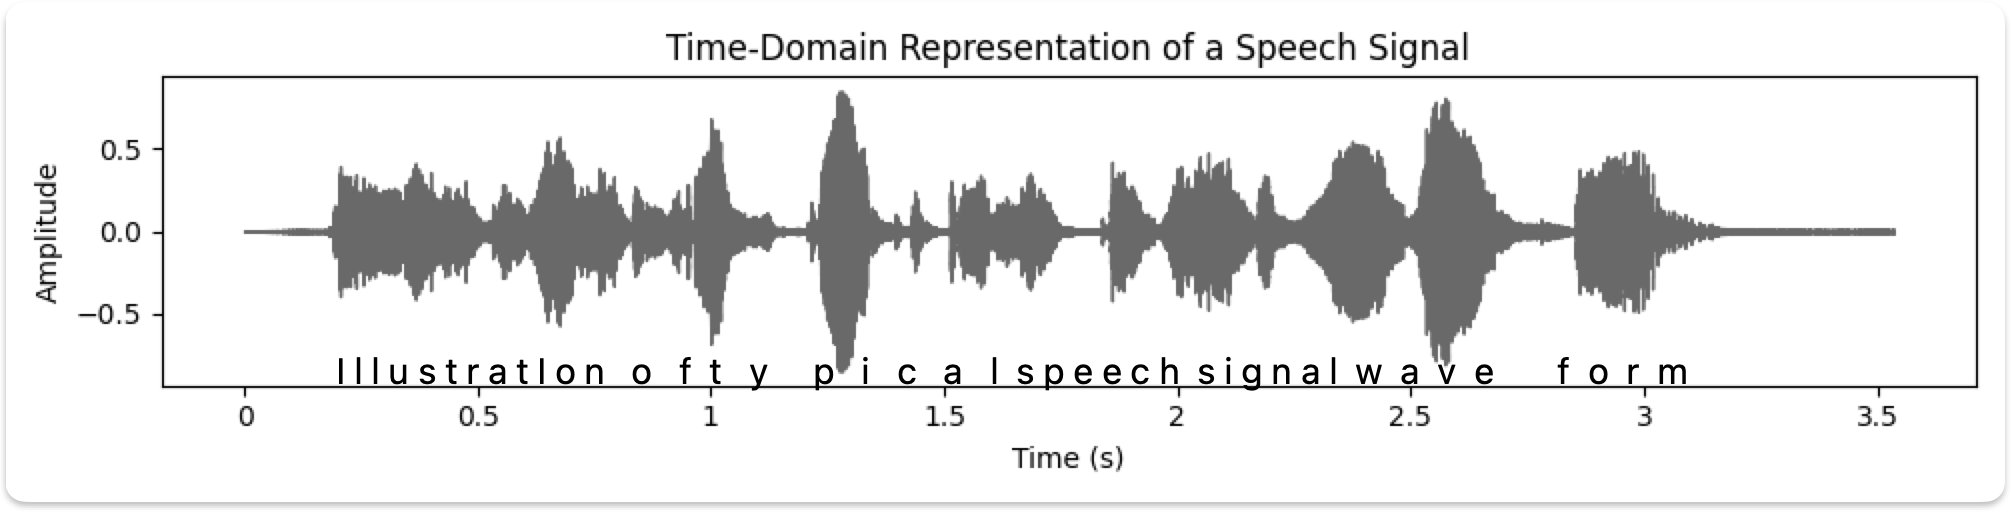
\includegraphics[width=.8\linewidth]{figures/figure7_waveform.jpg}
    \caption{Waveform of male voice.}
    \label{fig:figure1}
\end{figure}



\section{Fourier Transform (Frequency Domain Representation)}
While the time domain shows how the signal evolves over time, it does not reveal the frequency components that make up the signal.  
By applying the Fourier Transform (FT), the speech signal can be analyzed in the frequency domain, revealing which frequencies are present and their relative strengths.  
This is particularly important for understanding speech, as different sounds (such as vowels and consonants) occupy different frequency bands (Figure \ref{fig:figure2}). 


\begin{figure}[htbp]
    \centering
    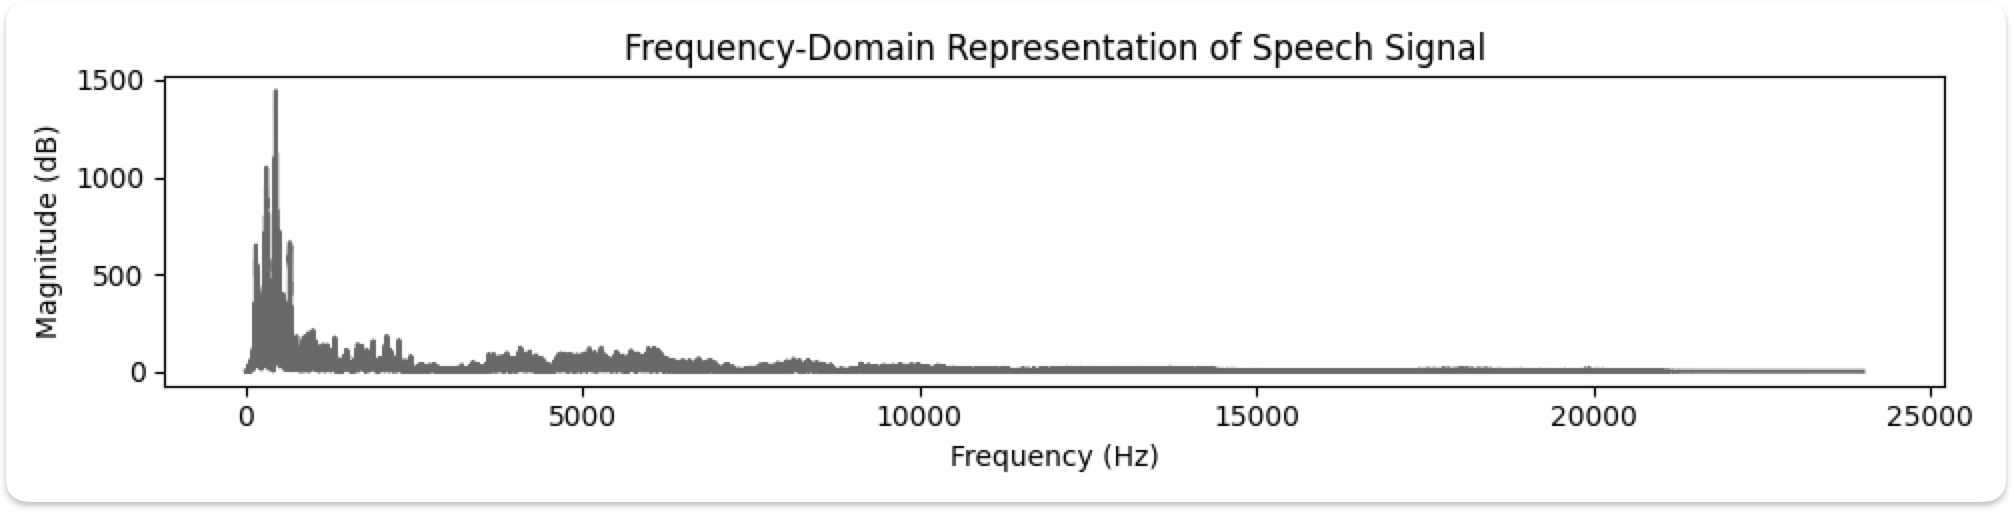
\includegraphics[width=.8\linewidth]{figures/figure8_1_fd.jpg}
    \caption{Speech Signal in a frequency domain.}
    \label{fig:figure2}
\end{figure}


\section{Spectrogram (Time–Frequency Representation)}

Speech signals are non-stationary, meaning their frequency content changes over time.
A spectrogram shows how the frequencies of a signal vary over time by applying the Short-Time Fourier Transform (STFT).

For machine learning applications, it is often better to use a Mel-Spectrogram (Figure \ref{fig:figure3}). Mel-Spectrograms are transformed spectrograms where frequencies are scaled to match how human ears perceive sound. After FT, it passes the result through a set of Mel filters that group frequencies in a way that matches how humans hear sounds.

Mel-Spectrograms represent the energy distribution of a speech signal across time and frequency and emphasize the perceptually important components of speech like formants (special frequencies that make each vowel sound different), harmonics (echoes of the main human voice pitch) and transitions between phonemes (single speech sounds, like "a", "s", "m") \cite{luitel2024audio}.


\begin{figure}[htbp]
    \centering
    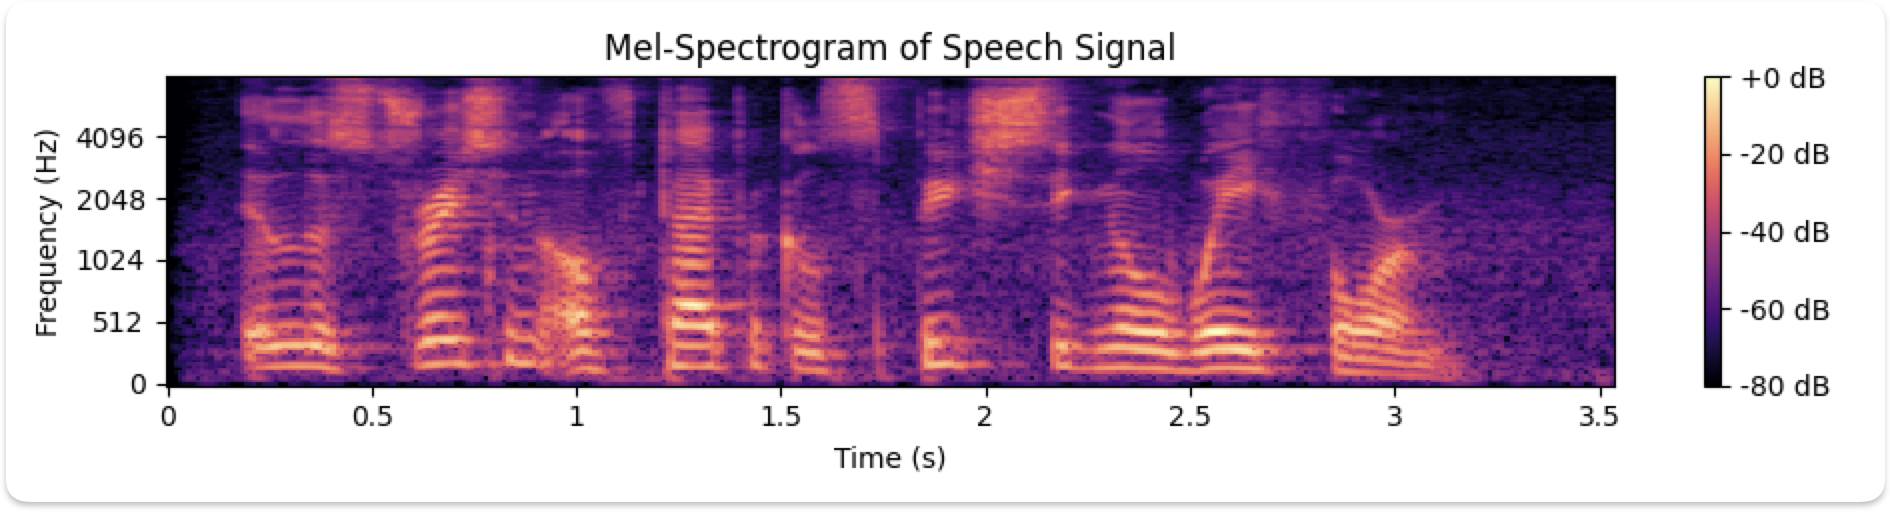
\includegraphics[width=.8\linewidth]{figures/mel-spectrogram.jpg}
    \caption{Mel-Spectrogram.}
    \label{fig:figure3}
\end{figure}


\section{The noise effect on speech signal}
As mentioned earlier, signal may be degraded or corrupted at various stages of speech signal processing. The illustration below clearly demonstrates how the signal from Figure \ref{fig:figure4} changes after the introduction of noise in the speech signal. The plot represents a continuous degradation of the signal.

\begin{figure}[htbp]
    \centering
    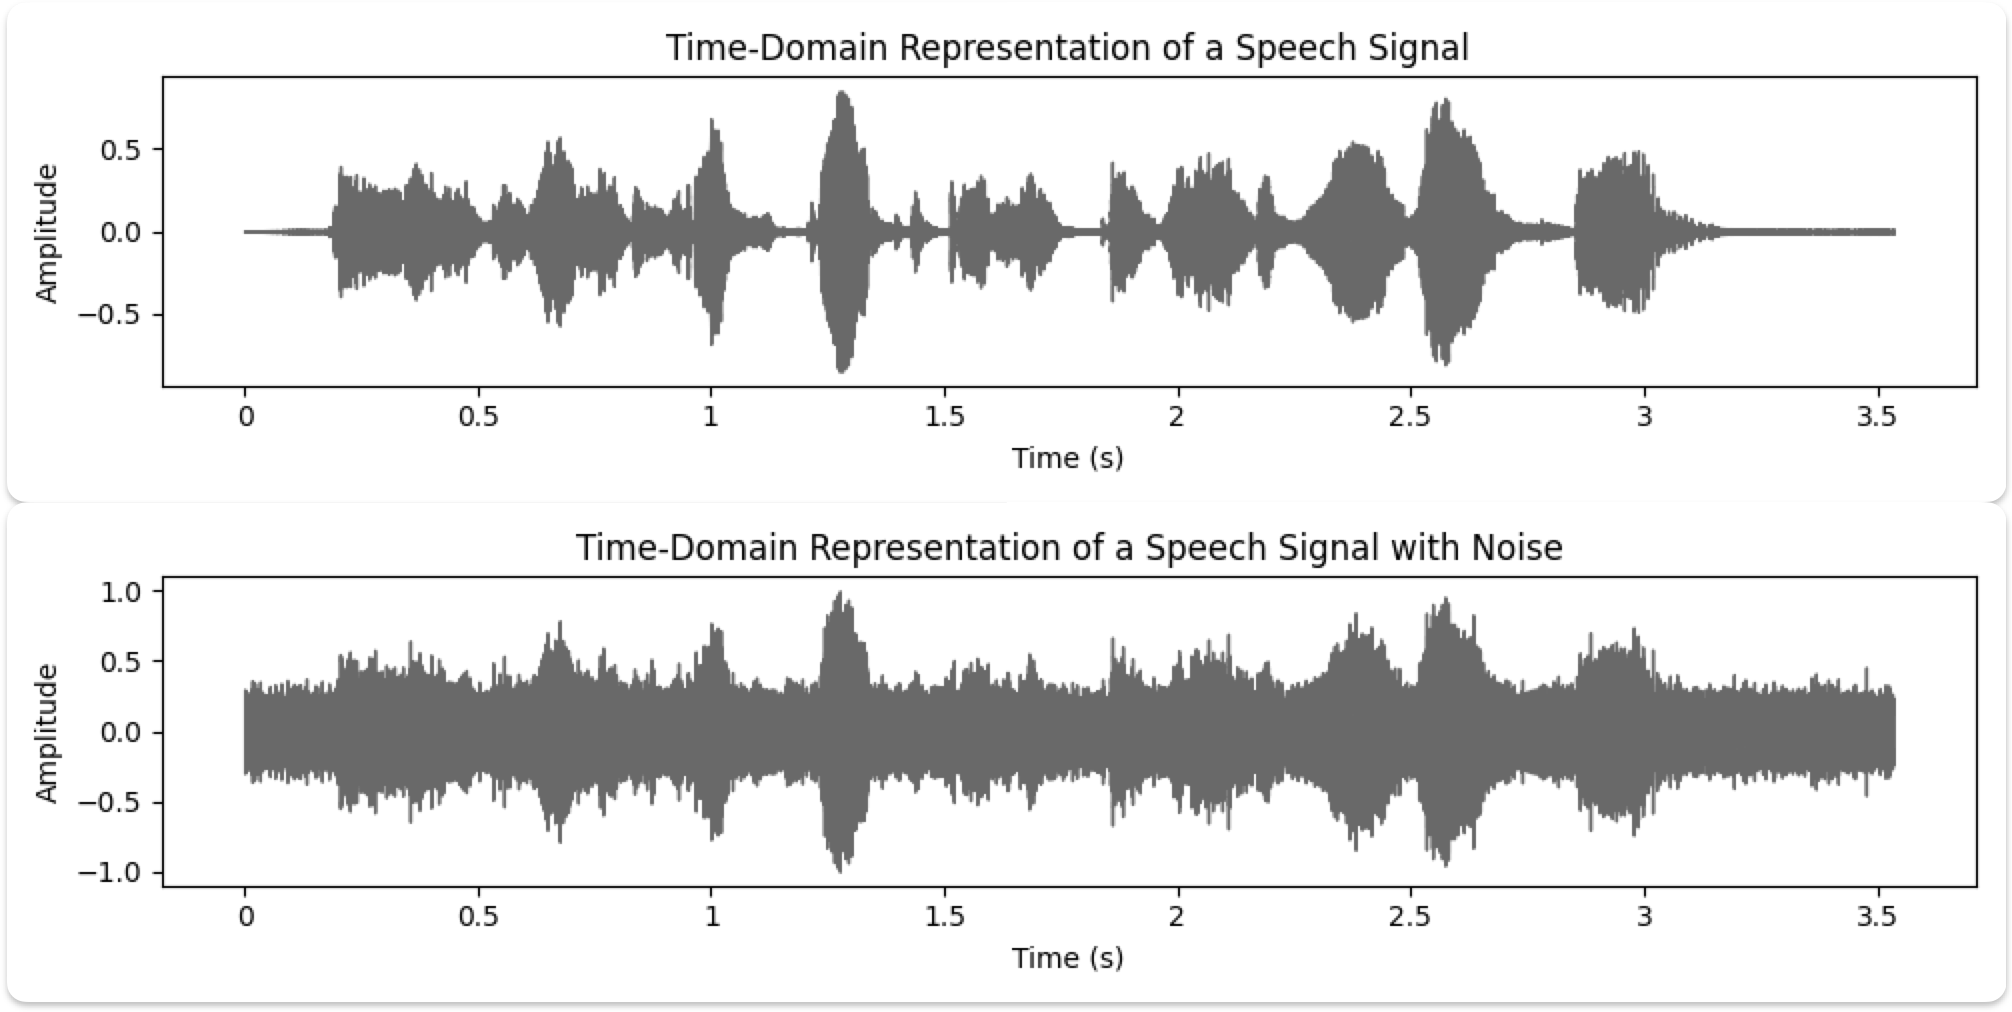
\includegraphics[width=0.8\linewidth]{figures/signal-with-a-gap.png}
     \caption{Waveform graphs of the original and noised signals.}
    \label{fig:figure4}
\end{figure}


The graph of the speech signal clearly shows changes compared to the original graph. 
 The lower waveform represents a case where the entire signal is covered by noise, masking the original speech content. When listening to the recording, the speech would sound distorted or buried under noise, making it difficult to perceive or understand. Such a signal disruption is unnatural and may occur due to environmental interference, low-quality recording conditions, or faulty equipment. Almost any part of the audio pipeline can contribute to this issue.
The loss of the audio signal can significantly reduce sound quality, making it a critical issue.


\section{Audio Inpainting}

Audio restoration refers to reconstructing degraded or corrupted parts of an audio signal. Just as image restoration removes noise and artifacts to recover visual quality, speech restoration aims to enhance clarity and naturalness in audio that has been affected by noise or distortion. In many real-world scenarios, the speech signal is not missing entirely but is masked by continuous or non-stationary background noise. Rather than identifying and filling silent gaps, the restoration process involves estimating a clean version of the speech signal from its noisy counterpart. Deep learning models, such as MetricGAN, enable this by learning perceptual representations of clean audio and optimizing the output to sound natural and intelligible, even when the original signal is heavily corrupted \cite{miotello}.


% \section{Deep Learning for Audio Inpainting}

% Deep learning refers to the field of training large neural networks with multiple layers to learn complex data patterns and has become a powerful tool for solving complex problems in signal processing, including the restoration of missing parts in audio signals \cite{ai-blog}.


% Deep learning has shown great potential for restoring missing parts of audio signals. One example is the work by Marafioti et al.~\cite{marafioti}, who proposed a context encoder that learns from the surrounding time–frequency information of the Short-Time Fourier Transform (STFT) to predict missing segments. Their results showed that deep neural networks can outperform traditional methods in preserving the naturalness and continuity of audio.

% Another approach was proposed by Miotello et al.~\cite{miotello}, who used a deep prior technique, where the structure of a multi-resolution convolutional network helps guide the inpainting process. Their model was able to reconstruct missing audio fragments with high accuracy, even without needing large training datasets. 

% Both studies show the effectiveness of deep learning in solving the challenges of audio reconstruction.

\chapter{Speech Signal Enhancement Methods: MetricGAN and Wiener Filter}
A Generative Adversarial Network (GAN) consists of two parts:

The \textbf{generator} learns to generate realistic data. The generated samples serve as negative training examples for the discriminator.

The \textbf{discriminator} learns to distinguish the generator's fake data from real data. It penalizes the generator for producing unrealistic results.

At the beginning of training, the generator produces fake data, and the discriminator quickly learns to identify it as fake.
As training progresses, the generator improves and starts producing outputs that can fool the discriminator.
Eventually, if the generator trains well, the discriminator becomes less effective at distinguishing real from fake. It begins classifying fake data as real, and its accuracy decreases.

Both the generator and the discriminator are neural networks. The generator's output is directly connected to the discriminator's input. Through backpropagation, the discriminator's classification provides a signal that the generator uses to update its weights \cite{metricgan}.

\section{MetricGAN Architecture for Audio Inpainting}

MetricGAN is a generative adversarial network model specifically designed for speech enhancement and restoration tasks. Unlike traditional models that optimize for signal similarity or statistical loss functions, MetricGAN is trained to directly optimize perceptual quality metrics (e.g., PESQ, STOI) by mimicking human perception of audio quality. This makes it well suited for enhancing noisy speech, even if the signal is entirely covered by background noise.

In speech tasks, the input to MetricGAN is a spectrogram of the noisy audio, and the output is a cleaned (enhanced) version of the spectrogram. Figure \ref{fig:figure5} illustrates this architecture: the generator takes in a magnitude spectrogram of the noisy signal and produces an enhanced spectrogram. The discriminator then compares the enhanced output against clean reference samples and estimates how close the perceptual quality is.

\begin{figure}[htbp]
    \centering
    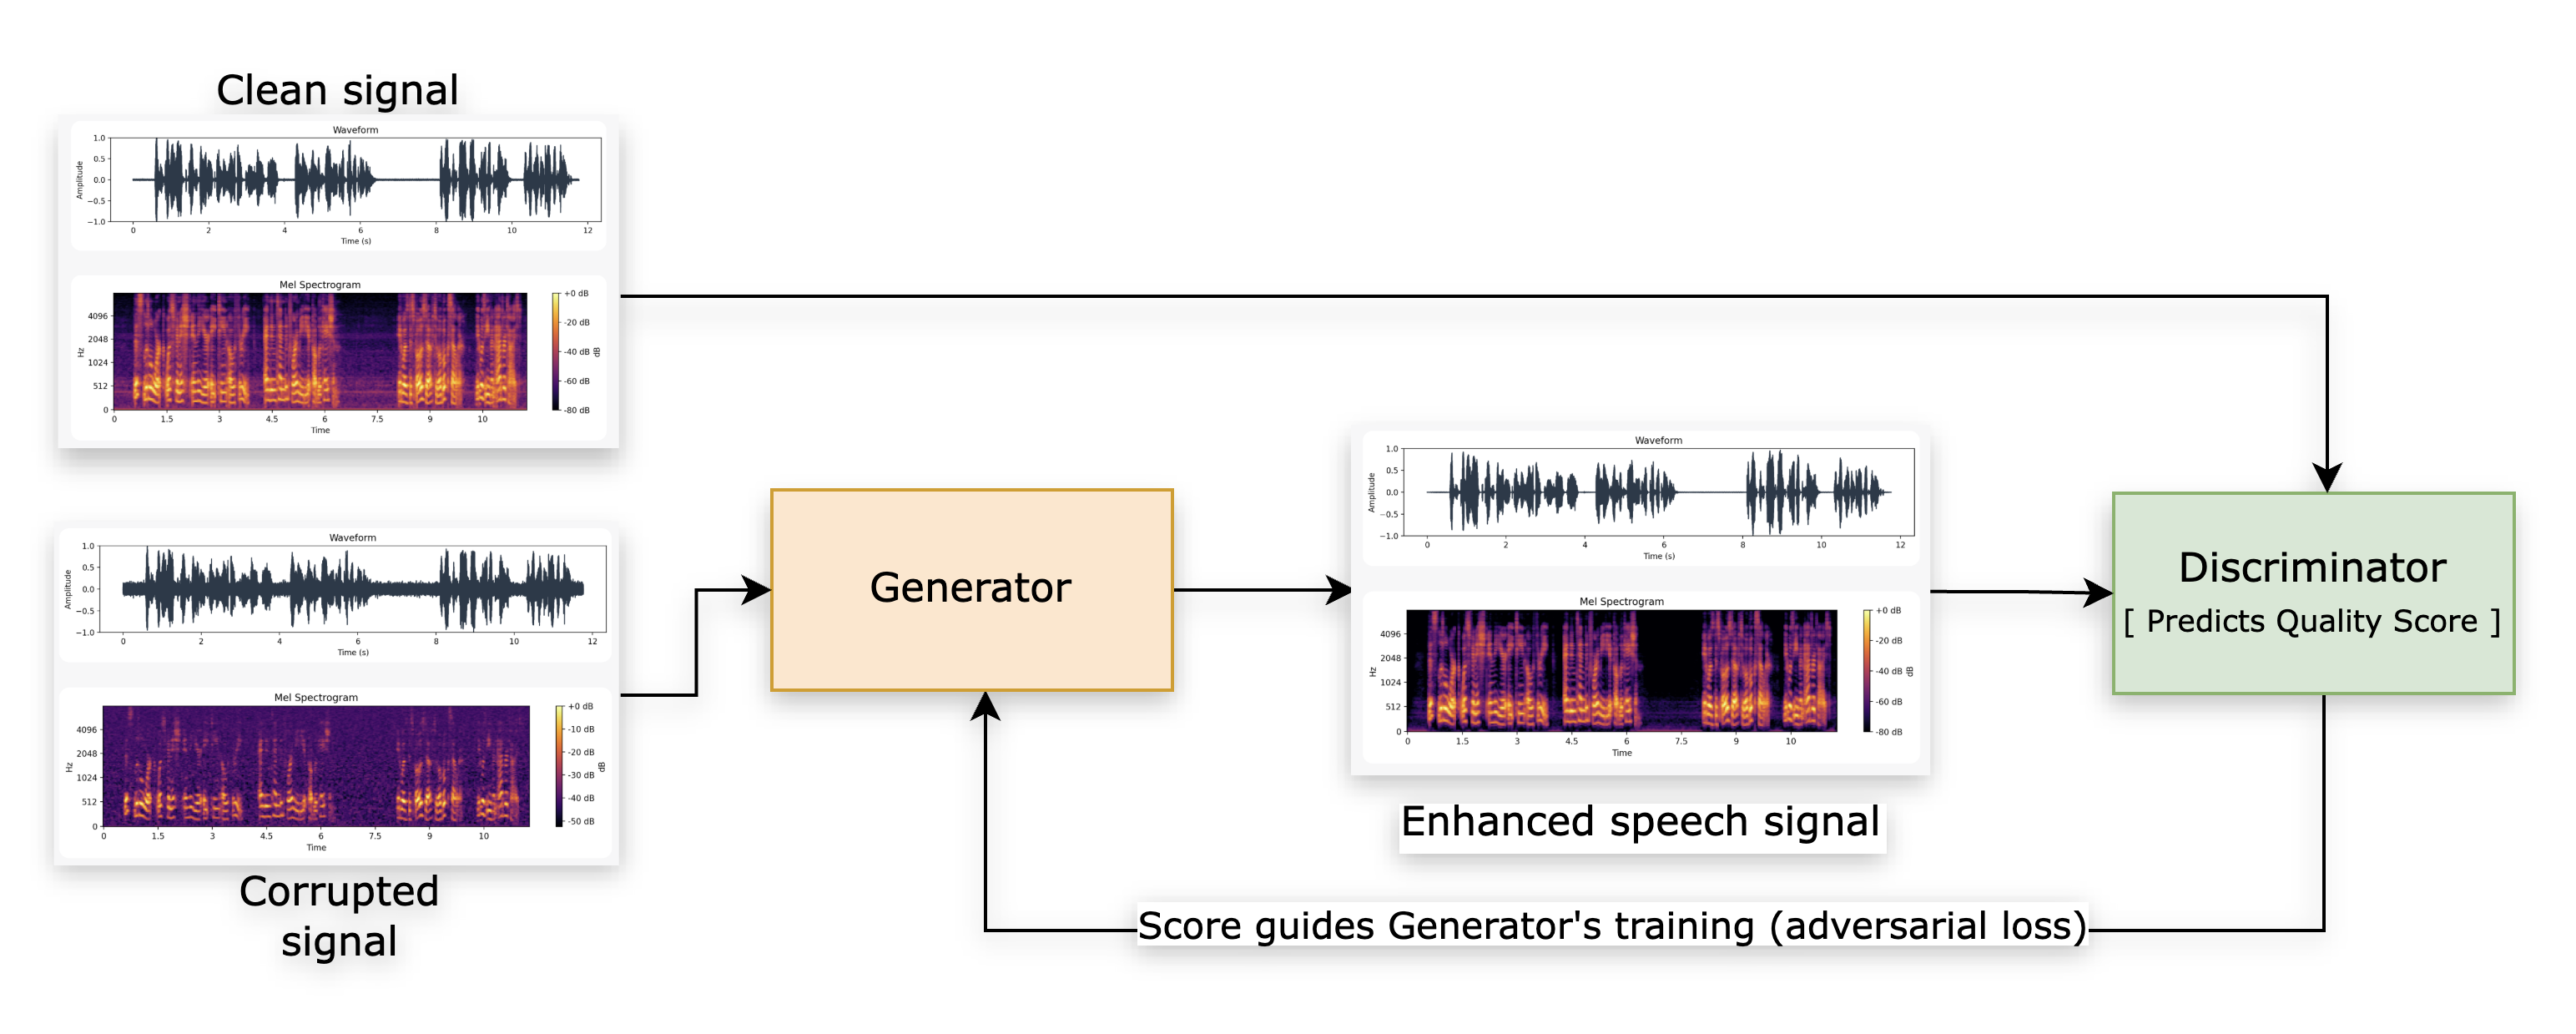
\includegraphics[width=1\linewidth]{figures/MetricGAN.png}
     \caption{High Level MetricGAN architecture. The generator produces enhanced audio, while the discriminator evaluates perceptual quality.}
    \label{fig:figure5}
\end{figure}

In a typical GAN structure, two neural networks - a generator and a discriminator — are trained in opposition. The generator learns to map a noisy audio input to its clean counterpart, while the discriminator evaluates how perceptually close the generated output is to a real, clean audio signal. What sets MetricGAN apart is that the discriminator is trained not just to classify real vs. fake, but to predict quality scores based on objective intelligibility and perceptual metrics.

Figure \ref{fig:figure6} illustrates the training process of the MetricGAN architecture, where the generator progressively enhances noisy speech signals. Over time, the quality of the enhanced output improves, as indicated by increasing PESQ scores: low (\(<\) 2.0), intermediate (2.0- 4.0), and high (\(>\) 4.0).

The generator produces enhanced audio from a corrupted input. This output is then evaluated by the discriminator, which predicts a perceptual quality score (PESQ) by comparing the enhanced signal to the clean reference. The predicted score is used to update the generator's parameters via adversarial loss, encouraging it to produce outputs that are perceptually closer to clean speech.

The discriminator plays a key role in guiding the generator’s learning, not by classifying real vs. fake, but by providing a continuous score that reflects human-perceived quality.


MetricGAN is widely used in modern speech enhancement benchmarks and has demonstrated strong performance in restoring intelligibility and perceptual quality, especially in real-world noisy environments where traditional gap-filling methods are ineffective. Its ability to learn perceptual optimization rather than just signal-level accuracy makes it especially effective for continuous signal degradation tasks.


\begin{figure}[H]
    \centering
    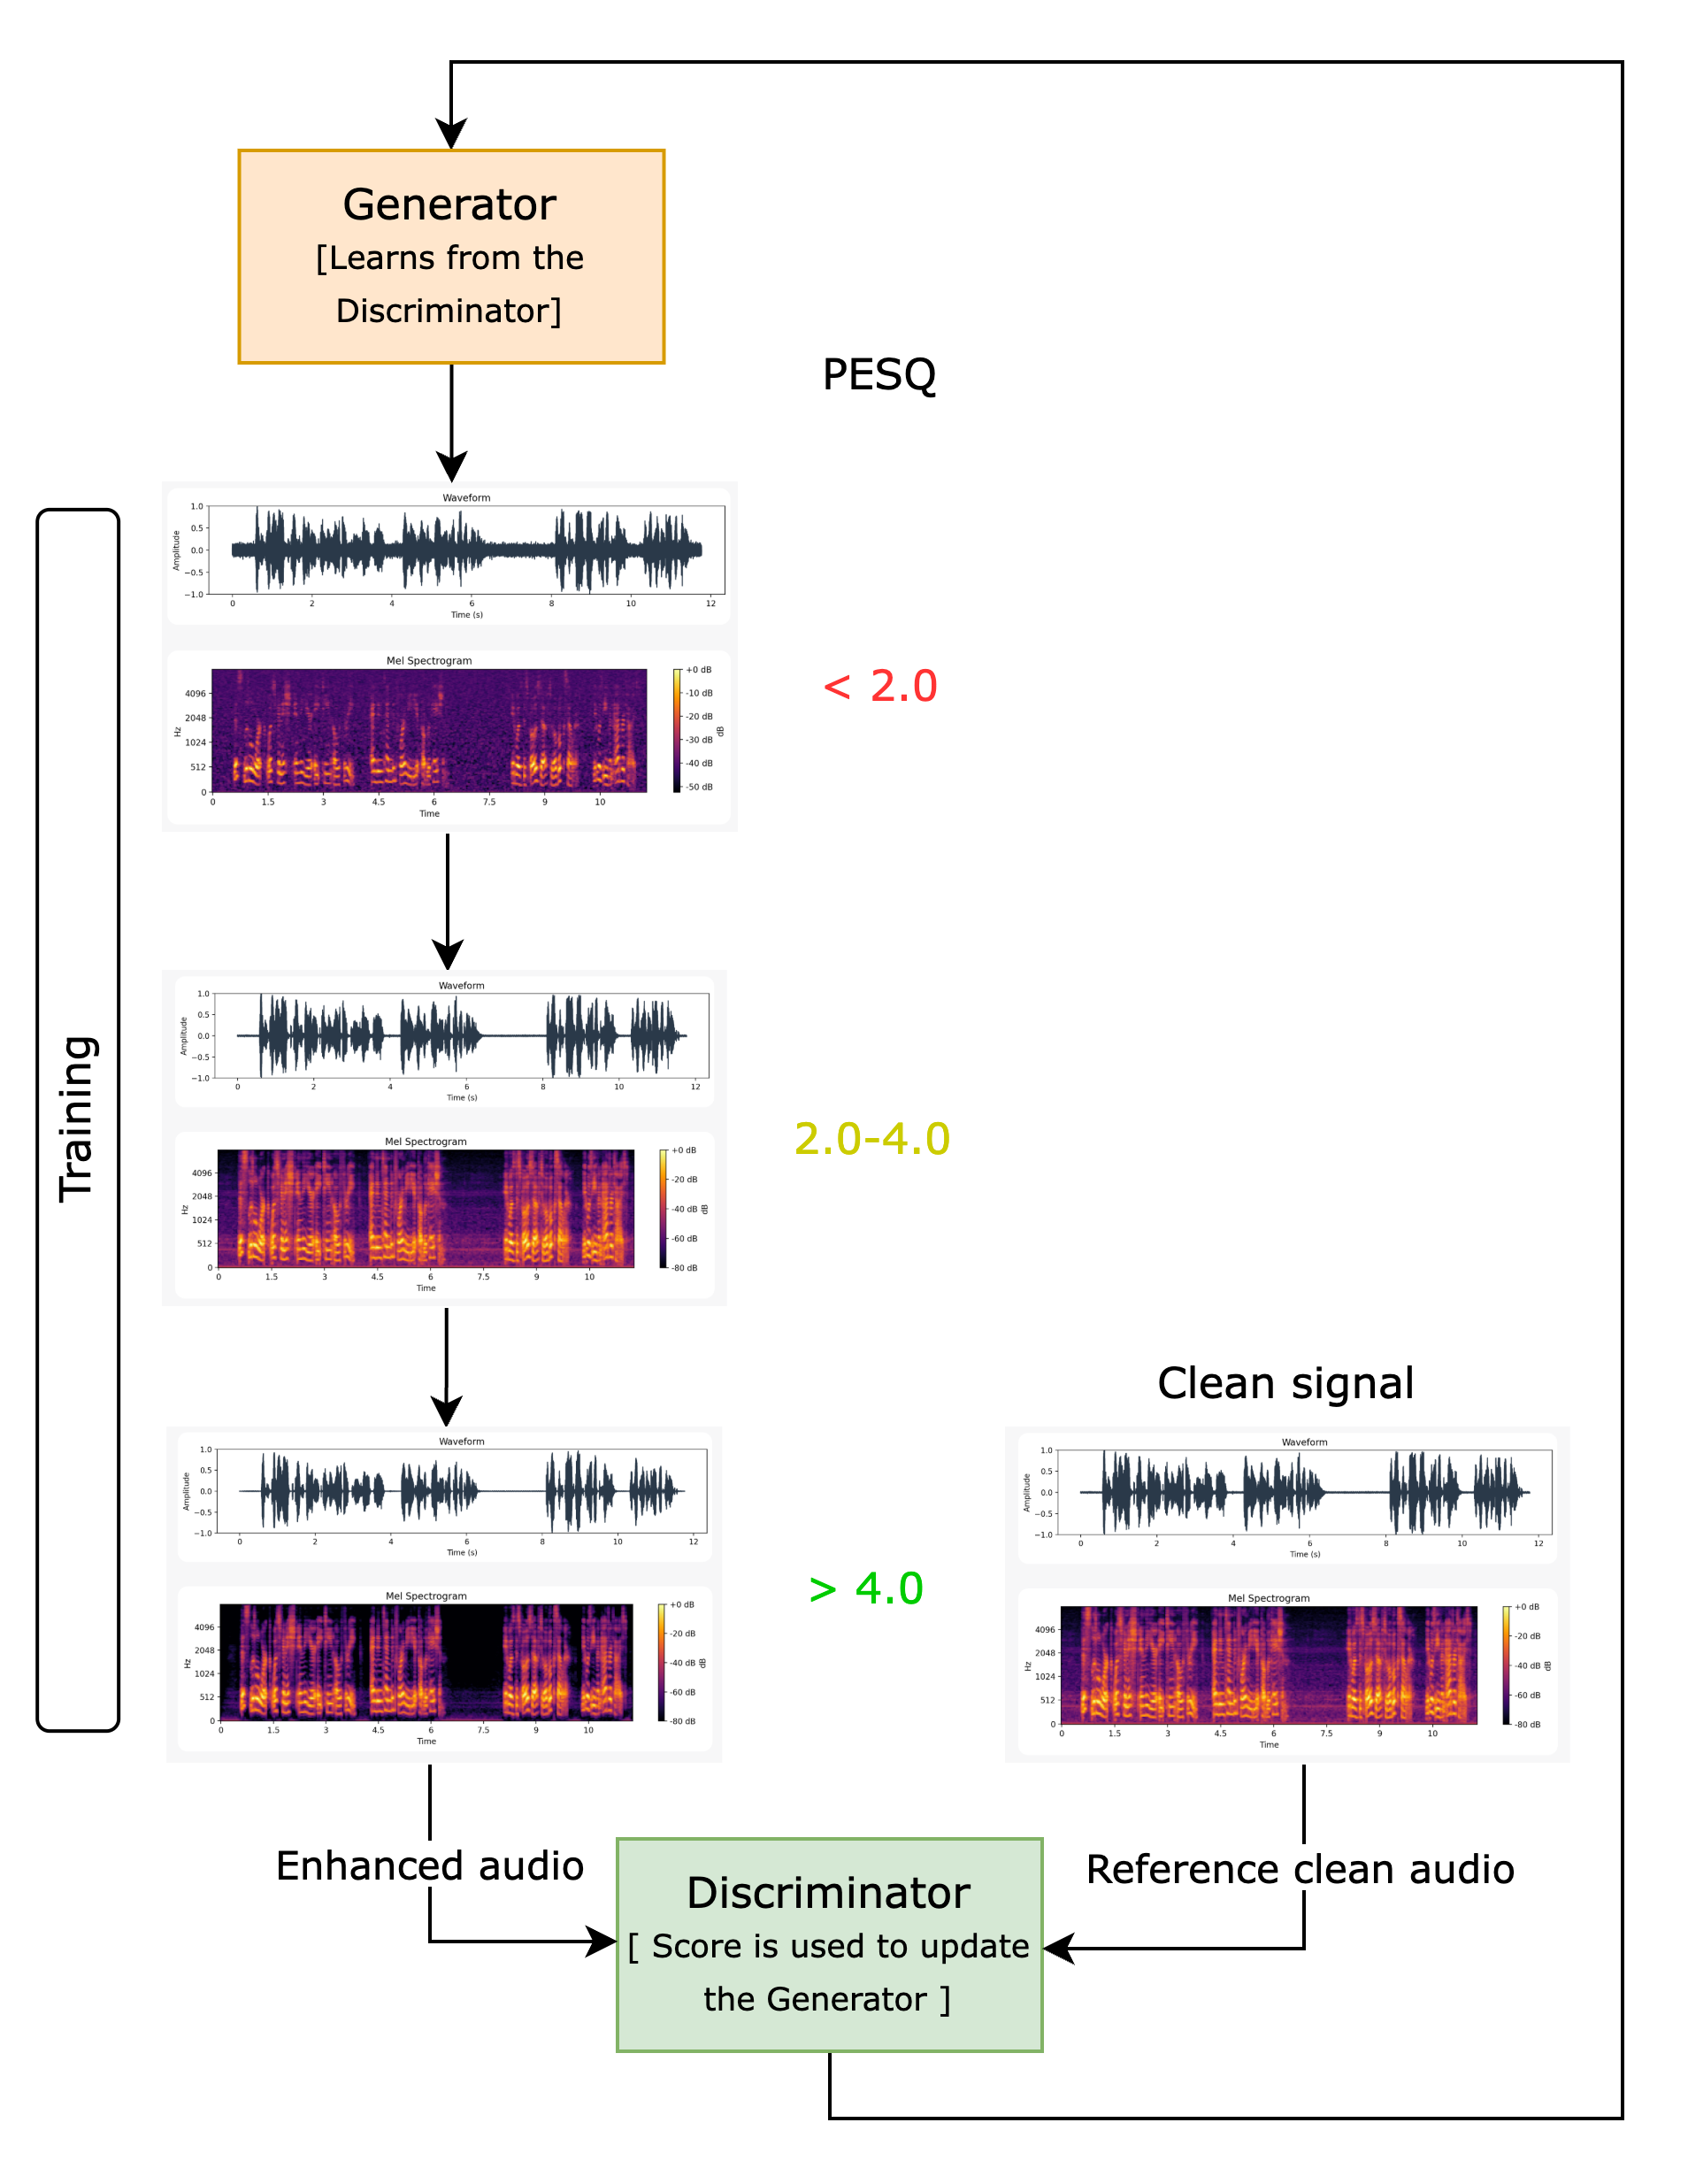
\includegraphics[width=.6\linewidth]{figures/gendis.png}
     \caption{MetricGAN Training Process Guided by PESQ Scores}
    \label{fig:figure6}
\end{figure}

\section{Wiener Filter for Speech Enhancement}

One of the classical approaches to speech signal reconstruction is Wiener filtering. Originally developed by Norbert Wiener, this method provides an optimal linear estimator of a clean signal from a noisy observation by minimizing the mean squared error (MSE).


In speech signal applications Wiener filtering is used to suppress noise and recover the clean speech. However, when noise is added, the clean and noisy components become dependent. As a result, the Wiener filter output contains both signals—typically with speech as the dominant component and noise as a residual minor part.

The Wiener filter works well when the noise level can be estimated accurately, usually during moments of silence in the recording. Its performance becomes worse when the missing parts are long or when the background noise changes over time. \cite{reddy}


Due to its historical importance and solid theoretical foundation, Wiener filtering has often been a baseline method in speech enhancement and restoration tasks. A detailed discussion of its application in speech processing can be found in the textbook by Loizou~\cite{loizou}, which remains one of the standard references in the field.

\chapter{Evaluation Metrics}

To objectively assess the quality of reconstructed speech signals, several evaluation metrics are commonly used. In this work, the reconstruction performance is measured using SNR, PESQ, and STOI.

\section{Perceptual Evaluation of Speech Quality}
PESQ - is an objective method used to assess the quality of speech signals after transmission or compression. It was developed to improve upon earlier models by accurately predicting perceived speech quality across a wide range of network conditions, including codec distortions, packet loss, filtering, and variable delays.

PESQ operates by comparing a reference (clean) speech signal with a degraded version. The perceived distortions are then calculated by analyzing the difference in loudness across time and frequency. These distortions are aggregated using a non-linear method known as the \(L_p\) norm:

\[L_p = (\sum_{m=1}^{M}disturbance[m]^p)^{1/p}\]
where \(m\) indexes the time-frequency cells.

The final step predicts the Mean Opinion Score (MOS), which represents the subjective quality of the speech, using a simple linear formula:

\[PESQMOS = 4.5 - 0.1 \times d_{sym} - 0.0309 \times d_{asym}\]
where \(d_{sym}\) and \(d_{asym}\) are asymetric disturbance parameters.

PESQ ranges from 1.0 (bad quality) to 4.5 (excellent quality). Higher values indicate better speech quality closer to natural, undistorted speech. \cite{pesq}

PESQ is an essential metric in this thesis because it provides an objective way to evaluate the quality of reconstructed speech signals. By comparing the restored speech to the original, PESQ helps determine whether the reconstruction methods preserve the naturalness and intelligibility of the speech as perceived by human listeners.


\section{Short-Time Objective Intelligibility}
STOI measure is an objective method designed to predict the intelligibility of speech signals, especially after noise reduction or time-frequency processing. Unlike traditional measures that focus on long-term signal statistics, STOI operates on short-time regions (approximately 400 ms) to capture local degradations in speech.

STOI is based on comparing the clean speech signal \(x\) and the processed (degraded) speech signal \(y\). Both signals are divided into overlapping short frames, transformed into the frequency domain using a STFT, and grouped into one-third octave bands. Within each short-time region, STOI computes a local normalized correlation between the clean and processed signals:


\[d_j(m) = corr(X_j(n), Y'_j(n))\]
where \(X_j(n)\) and \(Y'_j(n)\) are energy representation of the clean and processed signals for a specific frequency band and time frame, and \(Y'_j(n)\) includes normalization and clipping to stabilize distortions. 

The final STOI score \(d\) is obtained by averaging these local correlations over all time frames and frequency bands:


\[d = \frac{1}{JM}\sum_{j,m}d_j(m)\]
where \(J\) is the number of frequency bands and \(M\) is the number of time frames.

STOI scores range from 0 to 1, where 1 indicates perfect intelligibility and 0 indicates completely unintelligible speech. \cite{stoi}

STOI provides an objective way to measure how understandable the reconstructed speech signals are. Since this thesis focuses on restoring missing parts of speech, STOI helps evaluate whether the reconstruction preserves the original speech intelligibility. A higher STOI score after reconstruction indicates better performance of the proposed methods.



\section{Signal-to-Noise Ratio}

SNR - is a measure that compares the level of the desired signal to the level of background noise. It tells how much stronger the useful signal is compared to the unwanted noise. A higher SNR indicates that the reconstructed signal is closer to the original, with less distortion.

Mathematically, SNR is the ratio of signal power \(S\) to noise power \(N\), and is usually expressed in decibels (dB) using the formula:

\[SNR(dB) = 10\log_{10}{(\frac{S}{N})}\]

When signal and noise powers are given in dBm, SNR can be calculated by subtracting the noise level from the signal level. A higher SNR means better signal quality and less interference:
\[SNR(dB) = Signal(dBm) - Noise(dBm)\]

SNR scores range typically from low negative values (e.g., -10 – 30 dB). Higher SDR indicates that less distortion is present in the reconstructed signal compared to the original. \cite{snr}

In the context of this thesis, SNR is used as an objective metric to evaluate the quality of reconstructed speech signals. A higher SNR after reconstruction indicates a more accurate and effective restoration of the missing components.
\newpage

\chapter{Related Work}


\section{Introduction}
This chapter presents an overview of existing methods for reconstructing damaged or corrupted audio signals, covering both classical signal processing techniques and recent machine learning approaches. Special attention is given to deep learning models based on generative adversarial networks (GANs), which have shown strong performance in enhancing the perceptual quality of speech. The discussion includes the widely used classical Wiener filter, early deep neural network models, and modern GAN-based solutions such as MetricGAN.

Emphasis is placed on the comparison between classical and advanced machine learning approaches, with a focus on their strengths, limitations, and practical applicability for real-world speech restoration tasks. This review establishes the context for selecting MetricGAN as the core of the current system, as well as the evaluation strategies used to measure performance.


\section{Classical Baseline Methods}

In the work of Hilal H. Nuha et al.~\cite{nuha-noise-reduction}, Wiener filtering is applied as a classical technique for speech enhancement under conditions of strong additive noise. The study evaluates the effectiveness of Wiener filtering by adding controlled levels of Gaussian noise to clean speech and then applying the filter to reduce noise. Performance is assessed using the mean squared error (MSE) between the filtered and original speech signals across a range of low signal-to-noise ratios (SNRs). The results indicate that Wiener filtering can noticeably reduce background noise and improve the clarity of speech, particularly in the non-speech regions. However, the method becomes less effective as noise levels increase and SNR decreases, highlighting its limitations in highly adverse or rapidly changing noise environments. These findings confirm that, although Wiener filtering remains a practical and efficient baseline, it faces challenges when applied to speech signals with very low SNR or dynamic noise conditions.

\vspace{1em}

A more advanced variation of the Wiener filter was introduced by Wageesha Manamperi et al.~\cite{gmm-manamperi}, who developed a multi-stage speech enhancement method based on Gaussian Mixture Models (GMMs) for low SNR environments. This technique models the power spectral densities of both speech and noise using GMMs, enabling adaptive noise suppression under non-stationary conditions. The enhancement process employs a parametric Wiener filter applied in multiple stages, where noise estimates are refined iteratively using GMM mean vectors. Evaluation on the TIMIT dataset, with various noise types and levels, demonstrates that the GMM-based approach achieves higher speech quality (PESQ) and intelligibility (STOI) compared to traditional Wiener filtering. The results highlight the effectiveness of combining classical filtering with statistical modeling, bridging the gap between conventional and modern machine learning-based speech restoration methods.

\section{Deep Learning Approaches}


In the work by Saleem et al.~\cite{saleem2018dnnlw}, a DNN-based supervised learning approach was proposed to enhance speech corrupted by speech-babble noise, one of the most challenging types of background noise. The method, called DNN-LW, combines a deep neural network with a less aggressive Wiener filtering layer. The DNN is trained to estimate the magnitude spectrums of clean speech and noise, and the Wiener filter is applied as a post-processing step to generate the final enhanced output. The system was evaluated using the Noizeus dataset at various SNR levels from –10dB to +10dB. Objective metrics such as PESQ,  speech distortion (SIG), residual noise (BAK), STOI, and SDR were used. Results showed that the proposed method outperformed baseline techniques like standard Wiener filtering, log minimum mean square error (logMMSE), and spectral subtraction (SS), delivering higher intelligibility and better perceptual quality in difficult noise conditions.

\vspace{1em}

In the study by Morrone et al.~\cite{morrone2021audiovisual}, the authors proposed a deep learning-based framework for audio-visual speech inpainting, which restores missing parts of speech signals using both the audio context and visual information from face landmarks. Their model used log-magnitude spectrograms and a stack of Bi-directional Long-Short Term Memory (BLSTM) layers to predict the missing time-frequency tiles. Additionally, they explored a multi-task learning (MTL) strategy that combines speech inpainting with phone recognition. The method was evaluated using standard metrics such as STOI and PESQ, Phone Error Rate (PER), and L1 loss. Results showed that the audio-visual model significantly outperformed audio-only baselines, especially on longer gaps up to 1600 ms. Adding visual information notably improved intelligibility and quality, demonstrating that vision is valuable in restoring speech with large missing segments. In contrast, TDNN-based approach focuses on short gaps, relying only on the audio context and using its ability to model local temporal structure efficiently.

\vspace{1em}

In the work of Schreibman et al.~\cite{schreibman2024frann}, a deep neural network called FRANN (Feature Restoration Additive Neural Network) was proposed to restore speech features that were degraded by traditional speech enhancement techniques. Their system was designed to follow a standard Wiener filter-based noise suppression module, aiming to improve speech intelligibility without increasing the noise level. The model combined convolutional layers with LSTM units in a U-Net structure and was trained on LibriMix data mixed with WHAM! noise. The evaluation was performed using scale invariant signal-to-distortion ratio (SI-SDR), PESQ, SDR, and signal-to-distortion ratio (SNR) metrics. Results showed that FRANN significantly improved SI-SDR and PESQ scores compared to the baseline system, demonstrating its effectiveness in restoring lost speech features in low-latency settings without affecting the residual noise.

\vspace{1em}

A notable example is the work by Marafioti et al.\cite{marafioti}, who proposed a DNN architecture for audio inpainting based on the surrounding time-frequency context. Their model processes the STFT representation of the audio and predicts the missing time–frequency coefficients by learning from the available context. The architecture combines convolutional layers and fully connected layers to effectively extract local and global features from the reliable parts of the signal. Two strategies were explored: reconstructing the complexe-valued TF coefficients directly and reconstructing only the magnitude spectrum with separate phase estimation. The model focusing on magnitude reconstruction demonstrated better results, outperforming traditional methods like linear predictive coding (LPC) in restoring naturalness and continuity of the audio signal.

\vspace{1em}

In the work of Sun et al.~\cite{sun2021rnn}, a recurrent neural network (RNN)-based speech enhancement method was developed for application in binaural hearing aid systems. The proposed architecture utilizes gated recurrent units (GRUs) to process binaural signals, extracting 55-dimensional feature vectors from each ear, including Bark-frequency cepstral coefficients and other auditory features. Separate GRU networks are trained on the signals from each ear before concatenation through a fully connected layer, allowing the model to preserve binaural cues. The method aims to achieve a balance between noise suppression and speech intelligibility, while maintaining low computational complexity suitable for real-time implementation on embedded devices and smartphones. Evaluation was conducted on datasets simulating various noisy environments, and the proposed method was compared to deep learning and statistical-model-based baselines such as rnnoise and FSGJMAP. Objective measures such as PESQ, STOI, and SNR showed that the RNN-based method provides a good balance between speech quality and intelligibility, making it suitable for hearing aid systems with limited resources.



\section{GAN-based Models}

In the work of Hung et al.~\cite{hung2024integrating}, a modern speech enhancement system was proposed for hearing aid applications by integrating noise classification and deep learning-based restoration. The system first employs a convolutional neural network (CNN) to classify environmental noise types from MFCC features with an average recognition accuracy of 92\%. Once the noise category is identified, the system uses a conditional Generative Adversarial Network (cGAN) based on the StarGAN architecture to enhance speech signals, conditioning the generator on the identified noise class. Experiments conducted on the VCTK dataset mixed with ten types of environmental noise at various SNR levels demonstrated that the StarGAN model effectively suppresses a wide range of noises. Objective evaluation using PESQ, STOI, and Mel-Cepstral Distortion (MCD) metrics showed that the system achieves lower distortion and improved speech quality compared to CycleGAN-based baselines, although some degradation of the speech signal itself was observed. These results show that combining noise type recognition with GAN-based enhancement can improve speech quality in real hearing aid systems.

\vspace{1em}

In the work of Phan et al.~\cite{phan2021selfattention}, the authors proposed a self-attention generative adversarial network (SASEGAN) for speech enhancement. Their approach improves on the original SEGAN by adding self-attention layers, which help the network better capture long-range dependencies in audio signals. The generator in SASEGAN uses an encoder-decoder structure with convolutional layers, and self-attention is applied at different points to improve how the model focuses on important parts of the input. Experiments on the Voice Bank dataset with various noise types and levels showed that SASEGAN achieves better results than the SEGAN baseline on objective measures such as PESQ, STOI, CSIG, CBAK, and COVL. These results suggest that adding self-attention helps GAN-based models produce clearer and more natural enhanced speech, even in challenging noisy environments.


\vspace{1em}

In the study by Xu et al.~\cite{xu2022vsegan}, a novel visual speech enhancement generative adversarial network (VSEGAN) was proposed to improve speech quality in noisy environments by integrating visual information from video frames. The VSEGAN framework combines a multi-layer feature fusion convolutional generator with a discriminator, both trained adversarially. The generator utilizes both the spectrogram of noisy speech and visual features extracted from facial video frames, processing these streams through separate audio and video encoders, followed by a fusion and decoding stage. The architecture is designed to effectively merge audio and visual cues, leveraging the invariance of visual speech properties to acoustic noise.

Training was performed on the GRID and TCD-TIMIT datasets with 12 types of real-world noise and variable SNRs, using PESQ and STOI as evaluation metrics. Experimental results demonstrated that VSEGAN outperformed traditional audio-only GAN models such as SEGAN, as well as other recent audio-visual speech enhancement methods, in both objective quality and intelligibility measures. These results show that using visual information with GANs can make speech enhancement much stronger, especially in difficult, noisy situations.

\vspace{1em}

In the work of Liu et al.~\cite{liu2020cpgan}, a Context Pyramid Generative Adversarial Network (CP-GAN) was introduced for speech enhancement. The main innovation of CP-GAN is its use of a densely-connected feature pyramid generator, which combines features from different levels to better capture both local and global information in speech signals. To further improve performance, the model uses a dynamic context granularity discriminator, which includes both a global discriminator (for whole audio) and a local discriminator (for random segments). This approach allows the model to remove noise more effectively, even when it is unevenly distributed across the audio.

CP-GAN was evaluated on the Voice Bank and Librispeech datasets, using common metrics such as segSNR, STOI, PESQ, and MOS-based measures. Results showed that CP-GAN outperforms previous GAN-based methods and also helps improve the results of speech recognition and speaker verification systems when using the enhanced audio. These findings suggest that combining hierarchical context information with GAN-based models can lead to more robust and high-quality speech enhancement.

\vspace{1em}

In the study by Faraji et al.~\cite{faraji2020afpgan}, a GAN-based speech enhancement system was introduced that uses audio fingerprinting features to improve both efficiency and performance. Instead of relying only on common features like the STFT or MFCC, the authors proposed combining MFCC with normalized spectral subband centroids (NSSC) and their temporal derivatives to create a compact feature set called AFPC. This feature set captures both the energy and the structure of speech formants, providing more robust and informative input for the GAN model. Experiments on the LibriSpeech dataset with various noise types and SNRs showed that the MFCC+NSSC combination achieved the best or near-best results in terms of PESQ, STOI, and SDR, while also significantly reducing memory use, training time, and model size compared to larger feature sets. These results suggest that combining audio fingerprinting features with GAN-based speech enhancement can make such systems more practical for real-time and embedded applications.


\section{Conclusion and Analysis}

The literature shows clear progress in speech signal restoration, moving from traditional signal processing methods to advanced deep learning and generative models. Classical approaches like the Wiener filter are simple and work well for steady noise, but often fail when noise is strong or changes quickly. Adding statistical models, such as GMM-based Wiener filters, helps adapt to some changing conditions but still struggles with very dynamic noise.

Deep learning has brought major improvements. DNN-based and hybrid systems, which combine neural networks with classical filters, are better at handling difficult noises and improve how speech sounds. Systems that use both audio and visual signals go even further, especially when large parts of the speech signal are missing.

Recent GAN-based models represent the latest developments. They learn more flexible and perceptually meaningful features, and new ideas like conditional GANs or special feature sets have made them practical for real-world use in hearing aids and phones.

However, each method has limitations. Classical models are fast and lightweight but less effective in tough situations. Deep learning and GAN-based approaches give better results but usually need large datasets and more computing power. GANs also face issues like training difficulty and the need for better ways to measure results.

The trend is toward data-driven models that directly improve how speech sounds to people, across many types of noise and damage. For these reasons, MetricGAN is chosen in this work, as it combines the advantages of GANs with the direct optimization of perceptual speech quality, addressing the main challenges found in previous research.
\newpage



\chapter{Methodology}
\paragraph{}

This chapter explains how a speech restoration system was built and evaluated using MetricGAN, a leading-edge deep learning model for improving audio quality. Instead of training a model from scratch, this project makes use of a pretrained MetricGAN model integrated into a simple-to-use software tool. This approach makes it possible to restore degraded speech signals without needing extensive computational resources.

The system is a web-based application designed to let users upload audio files that have noise or other distortions, and receive clear, enhanced speech in return. Along with the restored audio, the system also provides audio quality metrics, using the evaluation methods described earlier (such as PESQ, STOI, and SNR).

To help users see the value of modern machine learning, the system compares the quality of the improved audio from the MetricGAN model with the results of a classic Wiener Filter method. This side-by-side comparison gives users a better understanding of how advanced deep learning models perform against traditional approaches for speech restoration.

The frontend of the system, built with the Svelte framework, interacts with a Python-based backend using FastAPI. The backend processes the uploaded audio using the pretrained MetricGAN model from the SpeechBrain library. 

Svelte was chosen for the frontend because it is lightweight and makes building fast, interactive interfaces easy. FastAPI was selected for the backend as it is modern, fast, and works well with Python and machine learning tools. SpeechBrain was used because it provides ready-to-use, high-quality speech enhancement models. This setup makes advanced speech restoration accessible and practical for users, regardless of their technical expertise.

The following sections of this chapter provide more details about how the system is structured, explain the steps involved in processing audio data, describe how the MetricGAN model was integrated, and outline the procedures used to evaluate the system’s performance.

\section{System Overview}

The proposed speech restoration system is designed using a clear client-server structure, making it easy to use and efficient. It consists of two main parts: a user-friendly frontend and a backend processing server. This design enables users to easily access advanced speech enhancement capabilities powered by the MetricGAN model.

\subsection{Frontend (User Interface)}

The frontend is built as a web application using Svelte. It provides a straightforward interface, allowing users to:
\begin{itemize}
    \item Upload speech audio files that are noisy, degraded, or contain missing parts.
    \item View the uploaded audio through clear waveforms and mel-spectrogram visualizations.
    \item Start the audio enhancement process with a simple click.
    \item Listen to or download the restored audio once processed.
\end{itemize}

This design simplifies the user experience, enabling users to test and use advanced audio restoration technologies.


\subsection{Backend (Processing Server)}

The backend server is developed using the Python FastAPI framework. Its responsibilities include:

\begin{itemize}
    \item Receiving audio files from the frontend through HTTP requests.
    \item The server converts the audio to mono and normalizes the amplitude, ensuring consistency for further processing.
    \item Running the pretrained MetricGAN model provided by the SpeechBrain toolkit to enhance the audio.
    \item Waveform and mel spectrogram plots are created using Matplotlib and Librosa to help users visualize the input audio.
    \item Evaluates the audio file quality using the metrics mentioned above (in case the original audio track was uploaded).
    \item Sending the improved audio back and metrics to the frontend.
\end{itemize}


\begin{figure}[htbp]
    \centering
    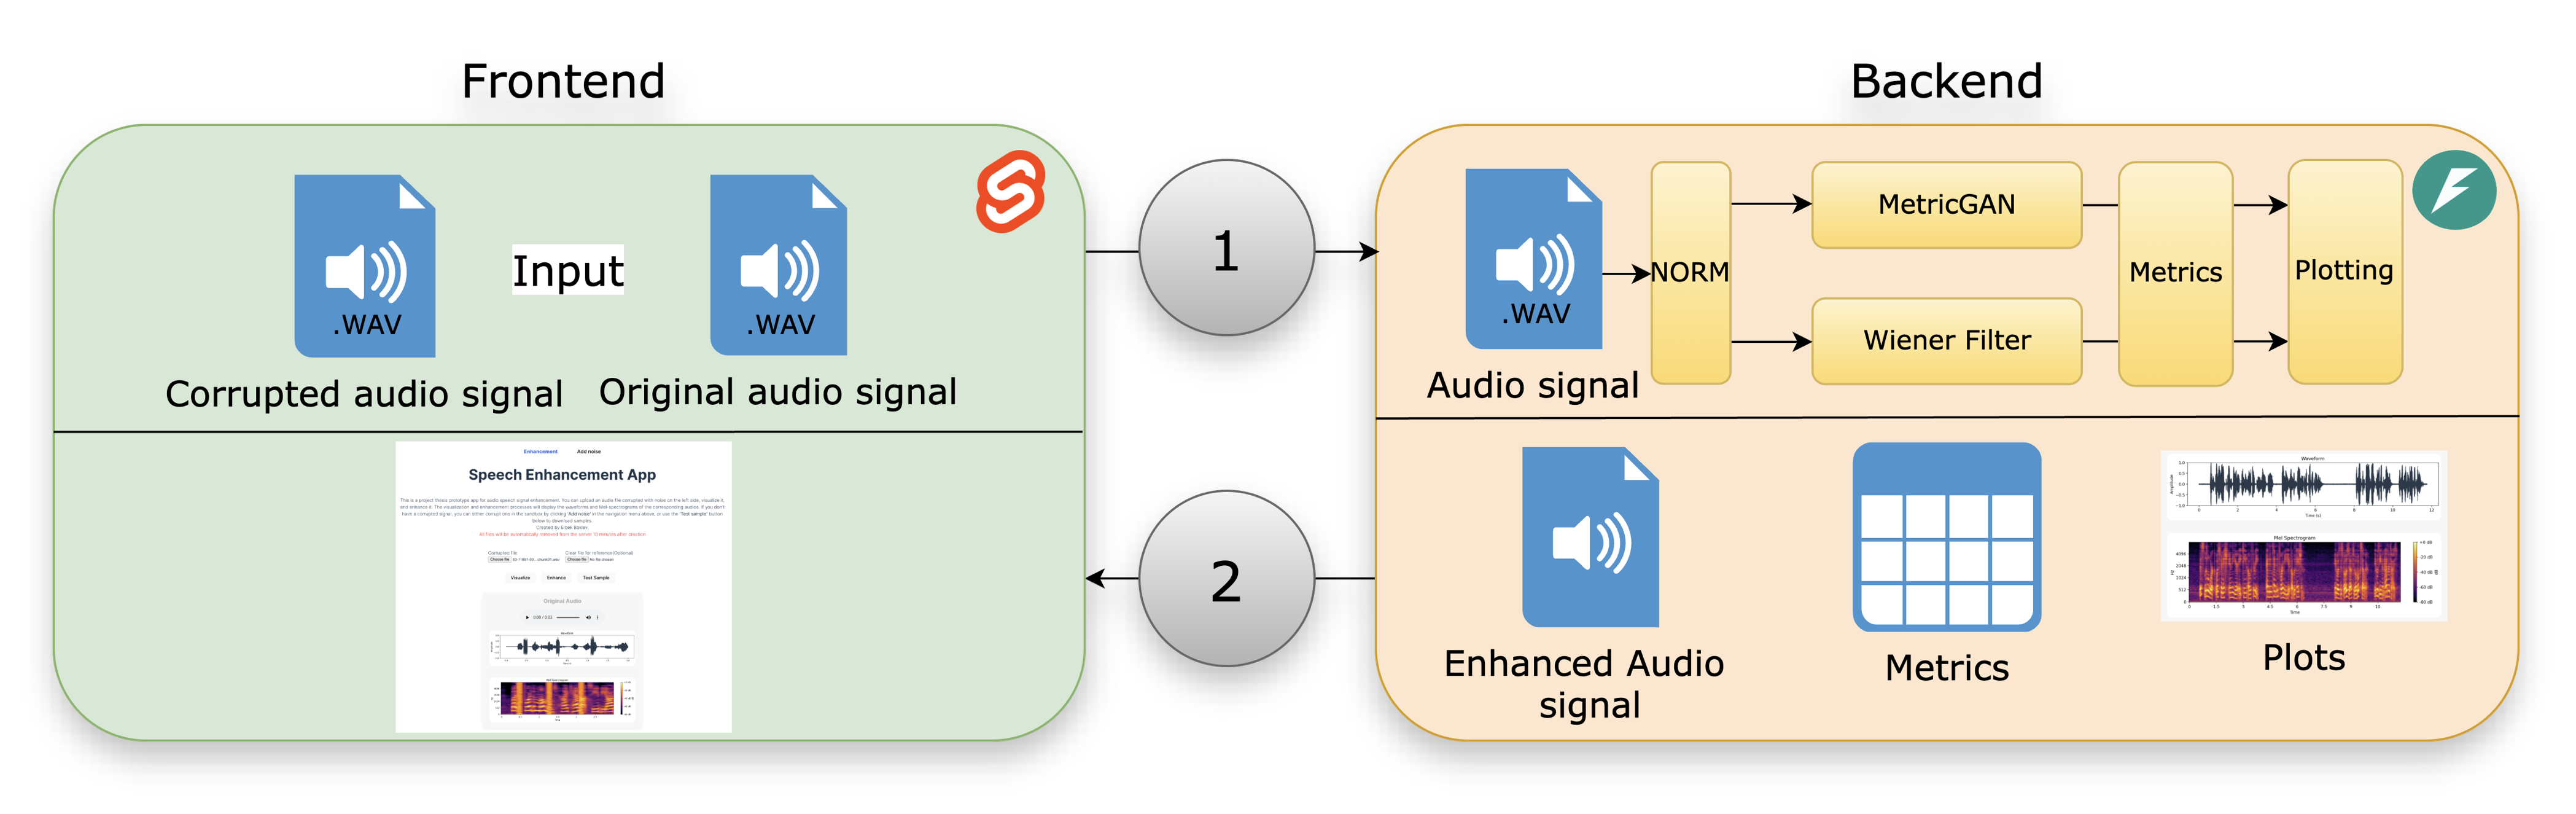
\includegraphics[width=1\linewidth]{figures/sysarch.png}
     \caption{System Architechture}
    \label{fig:figure7}
\end{figure}

Figure \ref{fig:figure7}  illustrates this workflow clearly, showing how the system can be interacted with, and model-based audio restoration is integrated.

\section{MetricGAN Model Details}
 This section summarizes the main architectural components and explains their roles in the speech enhancement process.
 
To better illustrate how MetricGAN works in practice, the core parts of the model’s code are shown in the appendix (see Appendix \ref{appendix:metricgan}) and presented in Figure \ref{fig:figure8}.

\subsection{Generator}
The generator’s job is to take the noisy or degraded audio features and predict what the clean features should look like. In MetricGAN, the generator is a neural network based on bi-directional LSTM layers (see Appendix \ref{appendix:metricgan}, lines 48-54)

\textbf{Input}: The input to the generator is a sequence of features extracted from the noisy audio (typically the magnitude spectrum).

\textbf{Processing:}

\begin{itemize}
    \item The sequence passes through two LSTM layers that capture both past and future context, which is important for modeling speech patterns.
    \item The LSTM output is processed by two fully connected (linear) layers with special initialization (Xavier for weights, zeros for bias).
    \item A custom “learnable sigmoid” activation function helps the network better map its outputs to realistic audio features.
\end{itemize}

\textbf{Output}: The generator predicts a mask or a set of features that can be used to reconstruct the enhanced audio signal.


\subsection{Discriminator}

The discriminator evaluates how close the enhanced output is to the clean reference, but in a way that relates to real perceptual audio quality metrics (see code in Appendix \ref{appendix:metricgan}, lines 77-124).

\textbf{Input}: The discriminator takes both the enhanced (fake) and clean (real) feature representations.

\textbf{Processing:}

\begin{itemize}
    \item The input first goes through batch normalization, followed by four convolutional layers
    \item Four convolutional layers extract spatial patterns from the audio feature maps, with activations and normalization to stabilize training.
    \item The output is averaged over time and frequency to summarize the features.
    \item Three linear layers reduce the dimensionality to a single score, which is used to estimate the perceptual quality (like PESQ).
\end{itemize}

\textbf{Output}: The final output is a single value that approximates the perceptual audio quality metric for the input.


\begin{figure}[htbp]
    \centering
    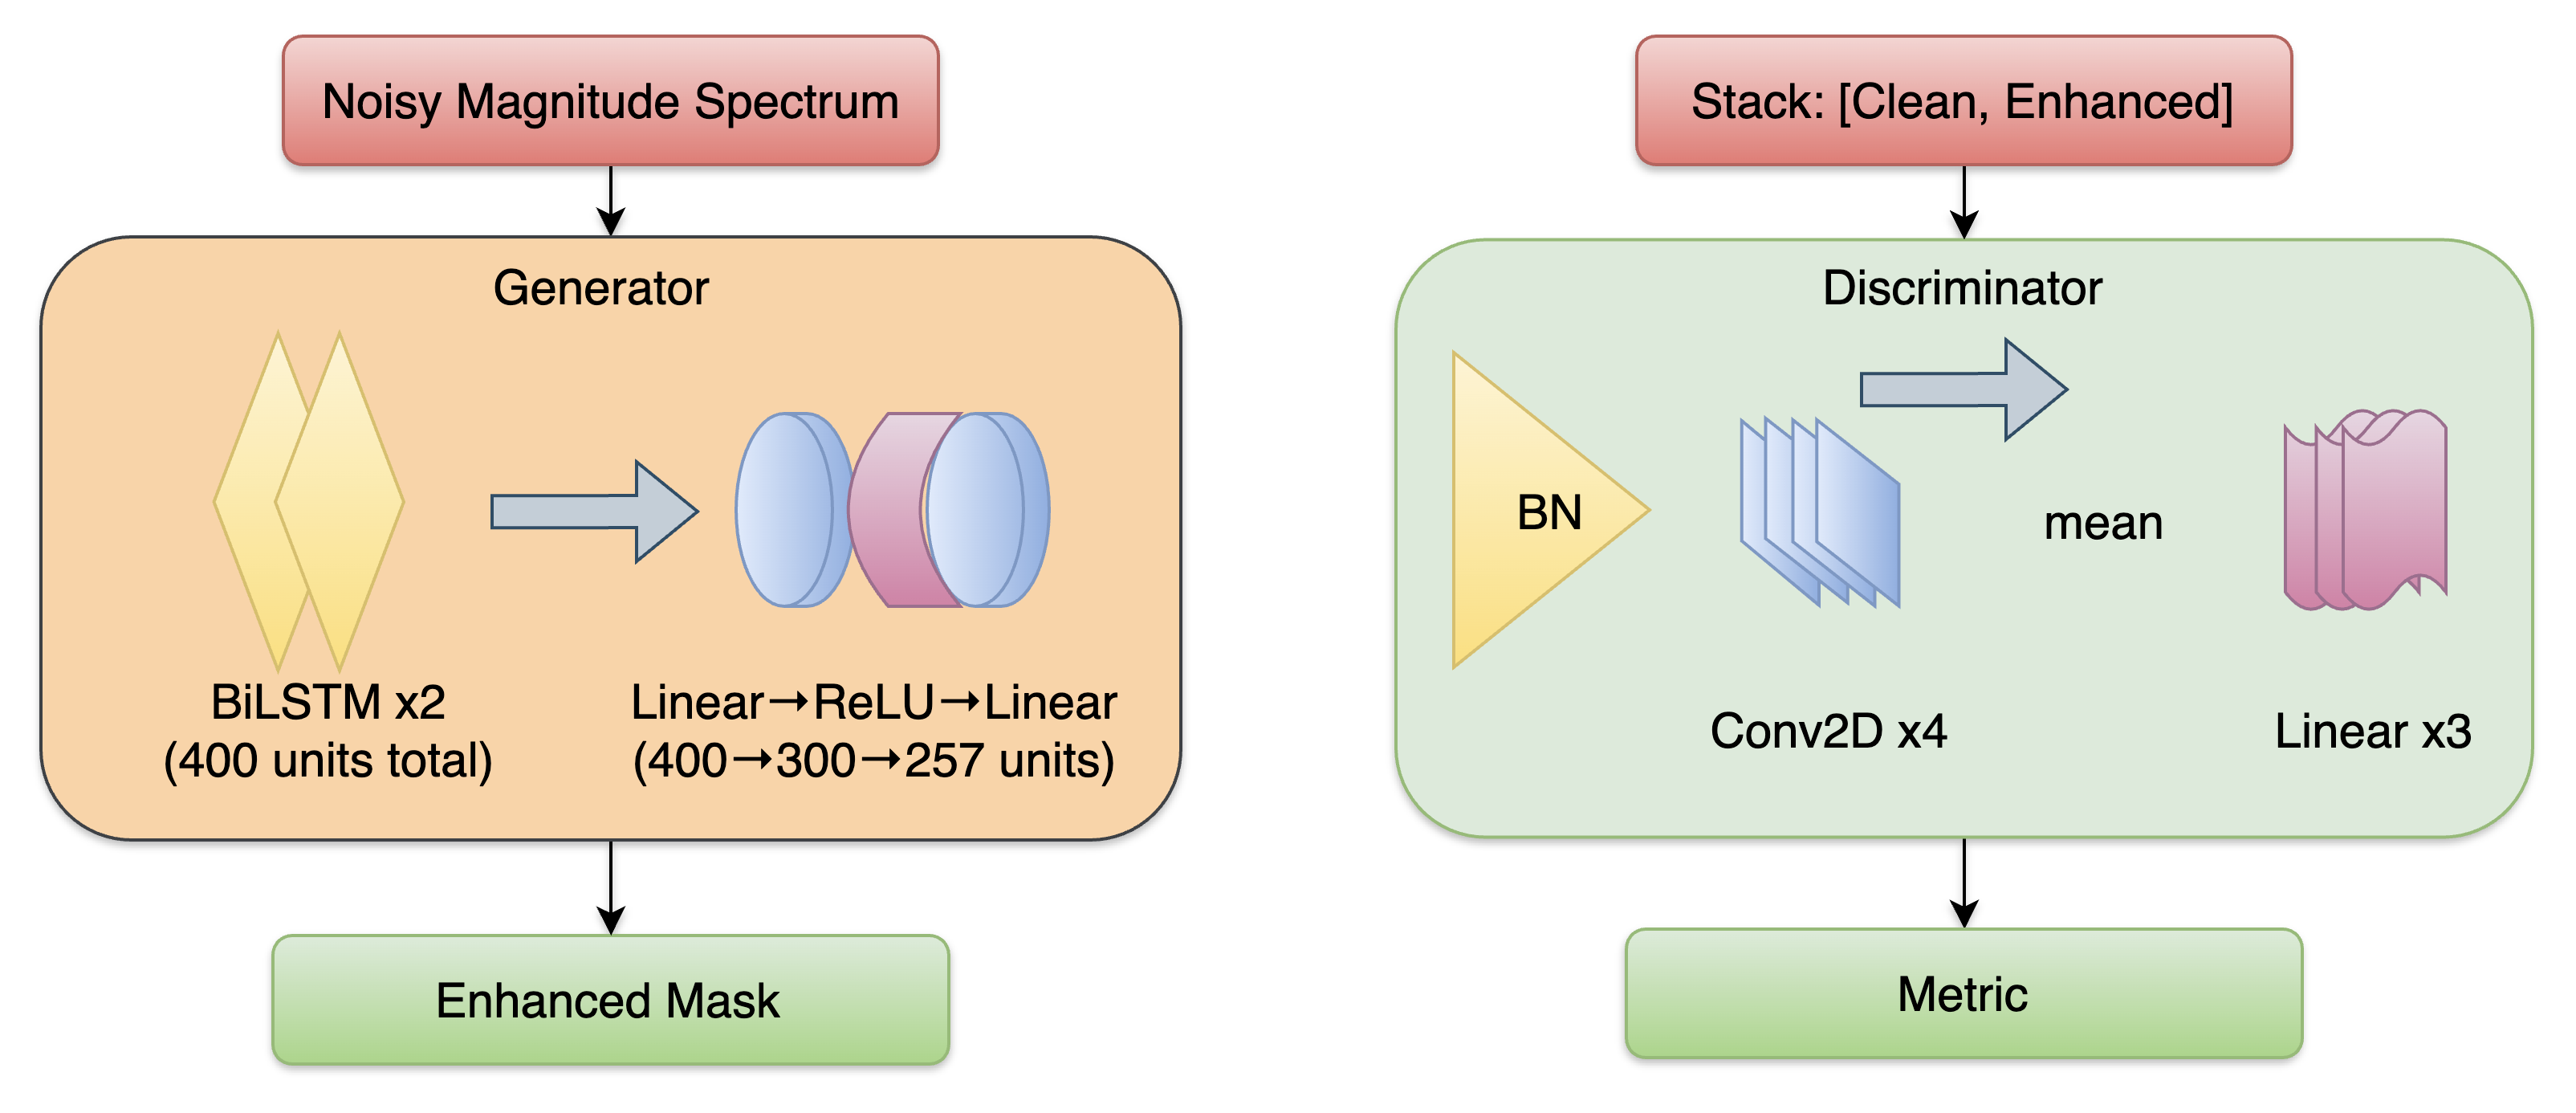
\includegraphics[width=1\linewidth]{figures/MetricGANCodeArch.png}
     \caption{MetricGAN Model Architecture}
    \label{fig:figure8}
\end{figure}


\subsection{Custom Components}

\textbf{Xavier Initialization and Spectral Norm}: The code uses custom helper functions to initialize neural network layers with “Xavier” initialization for weights and zero for biases, and optionally applies spectral normalization (see Appendix \ref{appendix:metricgan}, line 16).

\textbf{Learnable Sigmoid}: This is a special activation function where the “steepness” can be learned by the network, allowing more flexible outputs (see Appendix \ref{appendix:metricgan}, line 26).

\subsection{How the Model is Used in the System}
To use MetricGAN in the application, SpeechBrain’s inference wrapper was used (see Appendix \ref{appendix:metricgan_in_code})

This code loads the pretrained MetricGAN model and its parameters, making it ready for use on any uploaded audio file.

When an audio file is processed, the waveform is passed through the generator to create an enhanced version. During training, the discriminator would provide feedback on the perceptual quality, but for inference (in this project), only the generator is used to clean the audio.




\newpage

\chapter{Results and Analysis}
This chapter presents the experimental results for the proposed speech enhancement system. The performance of the MetricGAN-based method is evaluated and compared with the classical Wiener filter baseline, using both objective and perceptual speech quality metrics.

For the reference the figure representing original signal without noise is depicted below:
\begin{figure}[H]
    \centering
    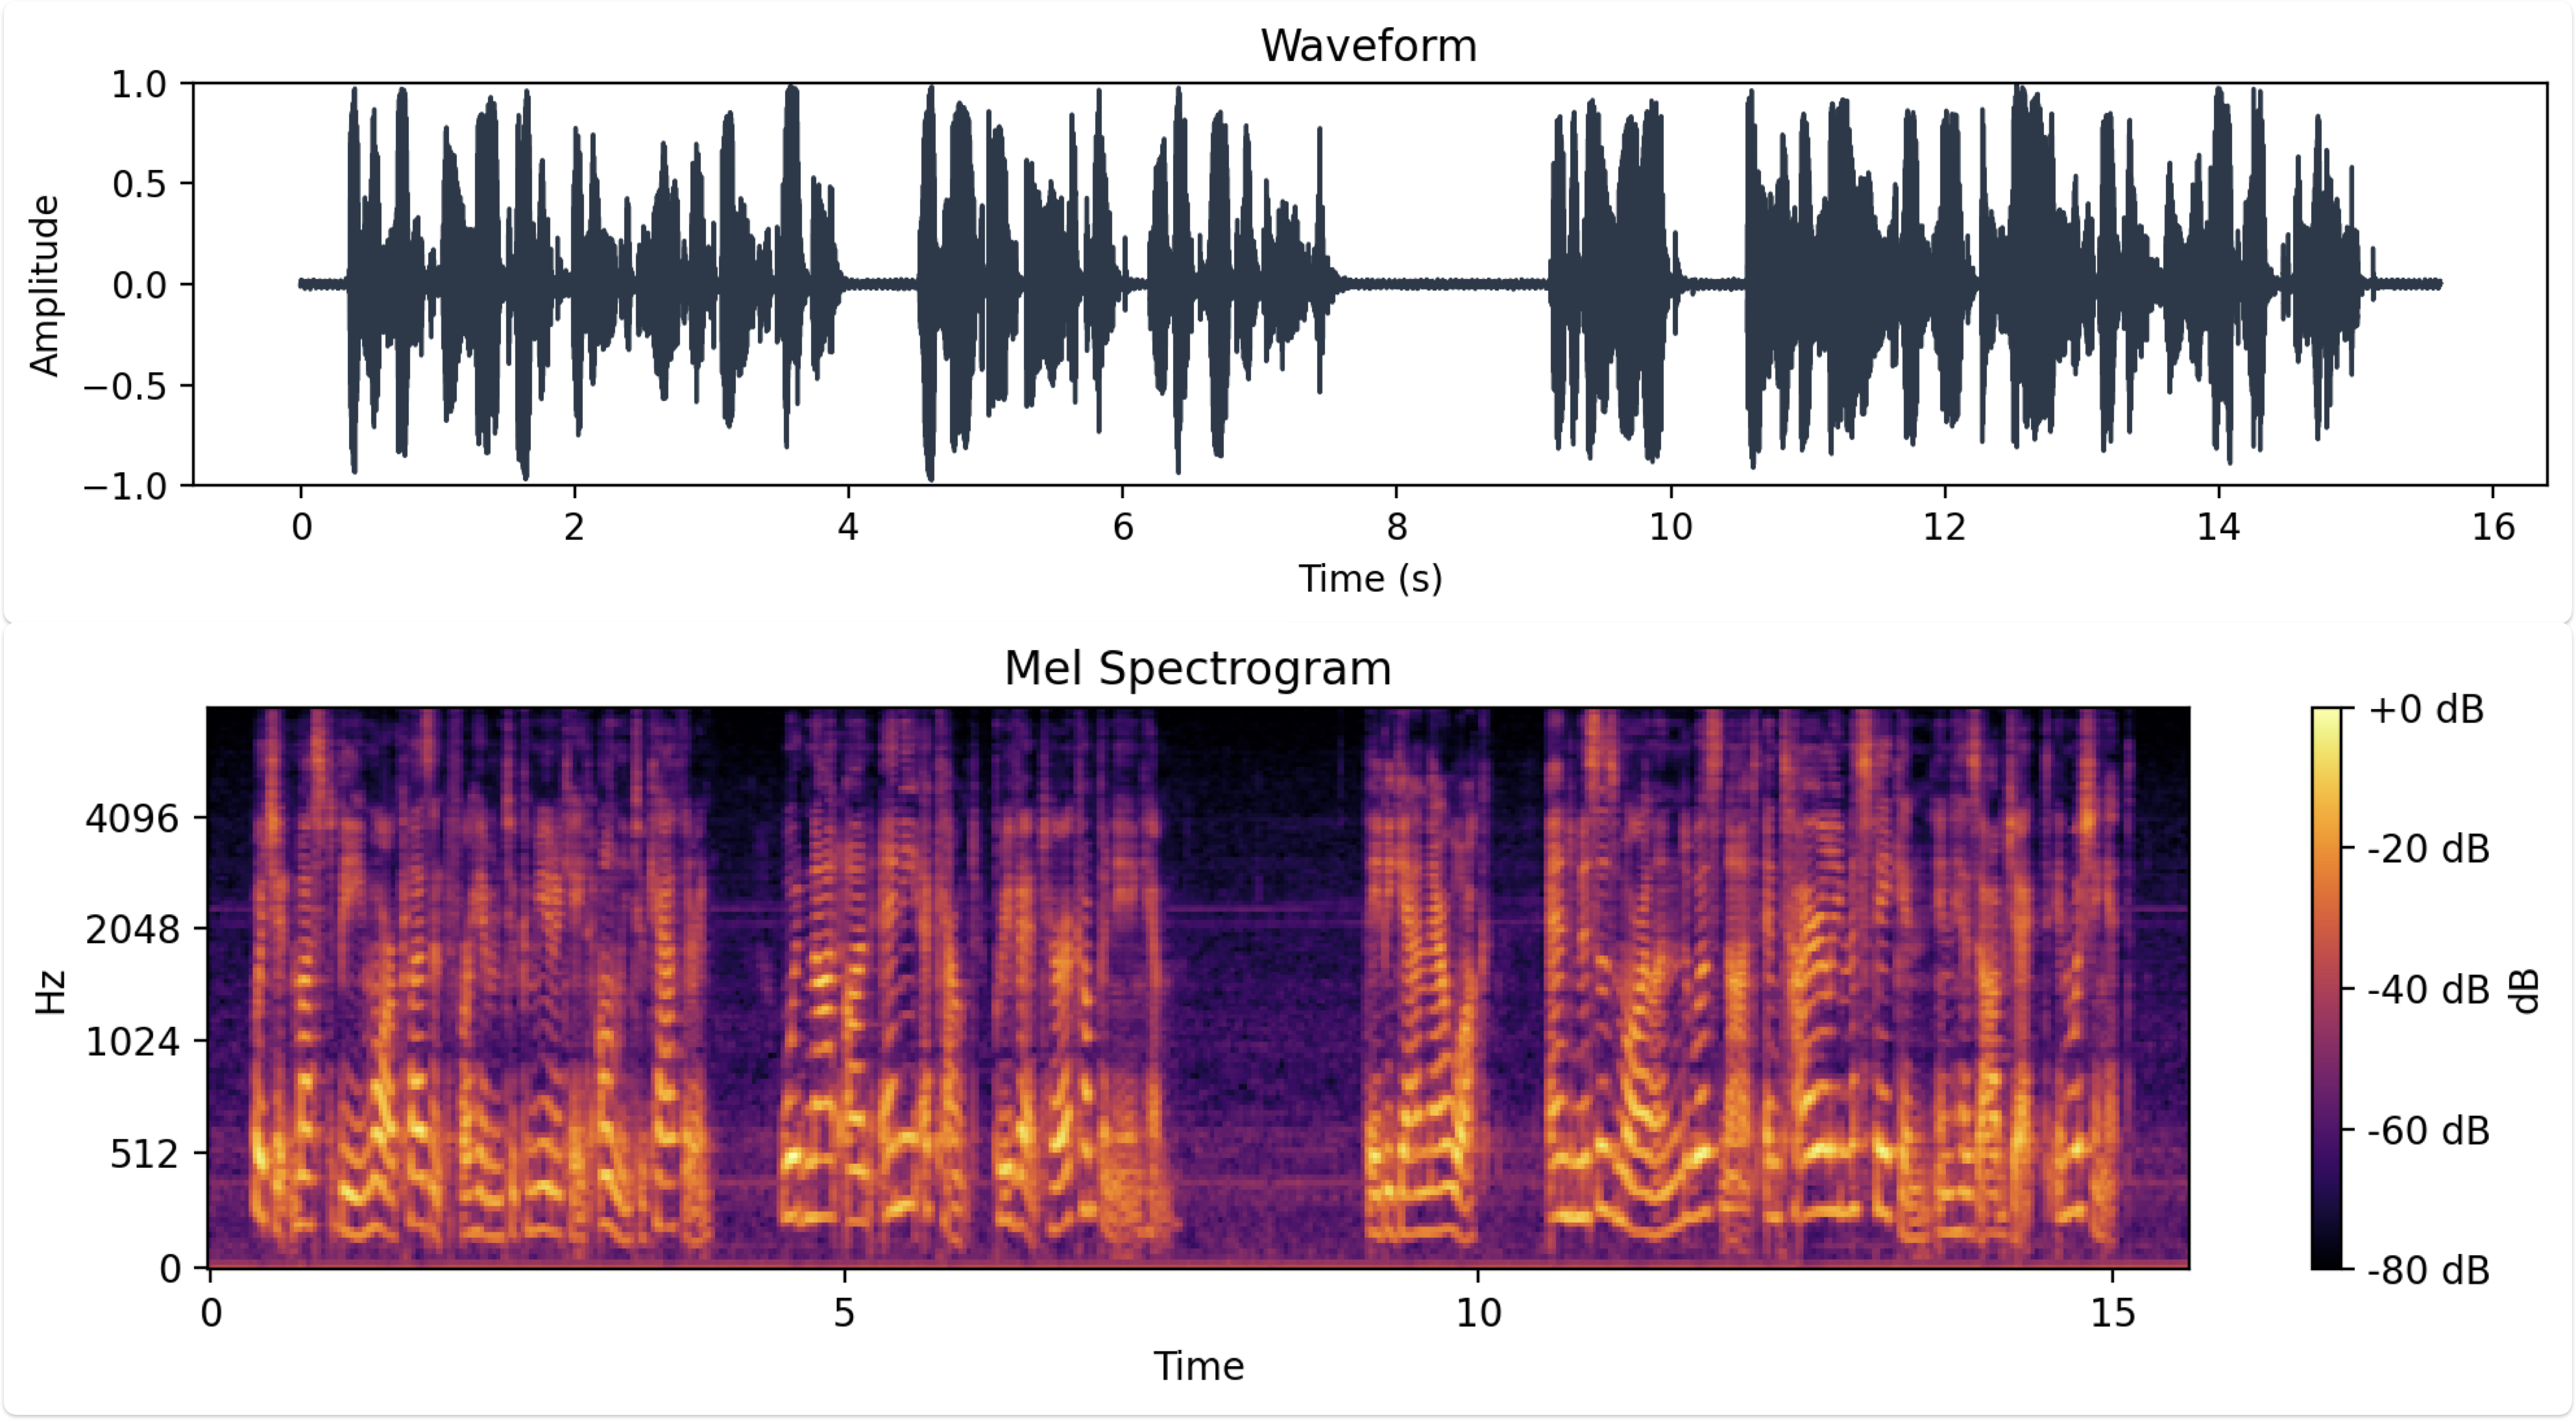
\includegraphics[width=.7\linewidth]{figures/original_.png}
     \caption{Original speech signal waveform}
    \label{fig:figure8}
\end{figure}



Sample was taken from LibriSpeech. Audio was affected by white noise with  0, 5, 10, 15, 20 SNR values. 


\begin{figure}[H]
    \centering
         \begin{subfigure}[b]{0.3\textwidth}
             \centering
             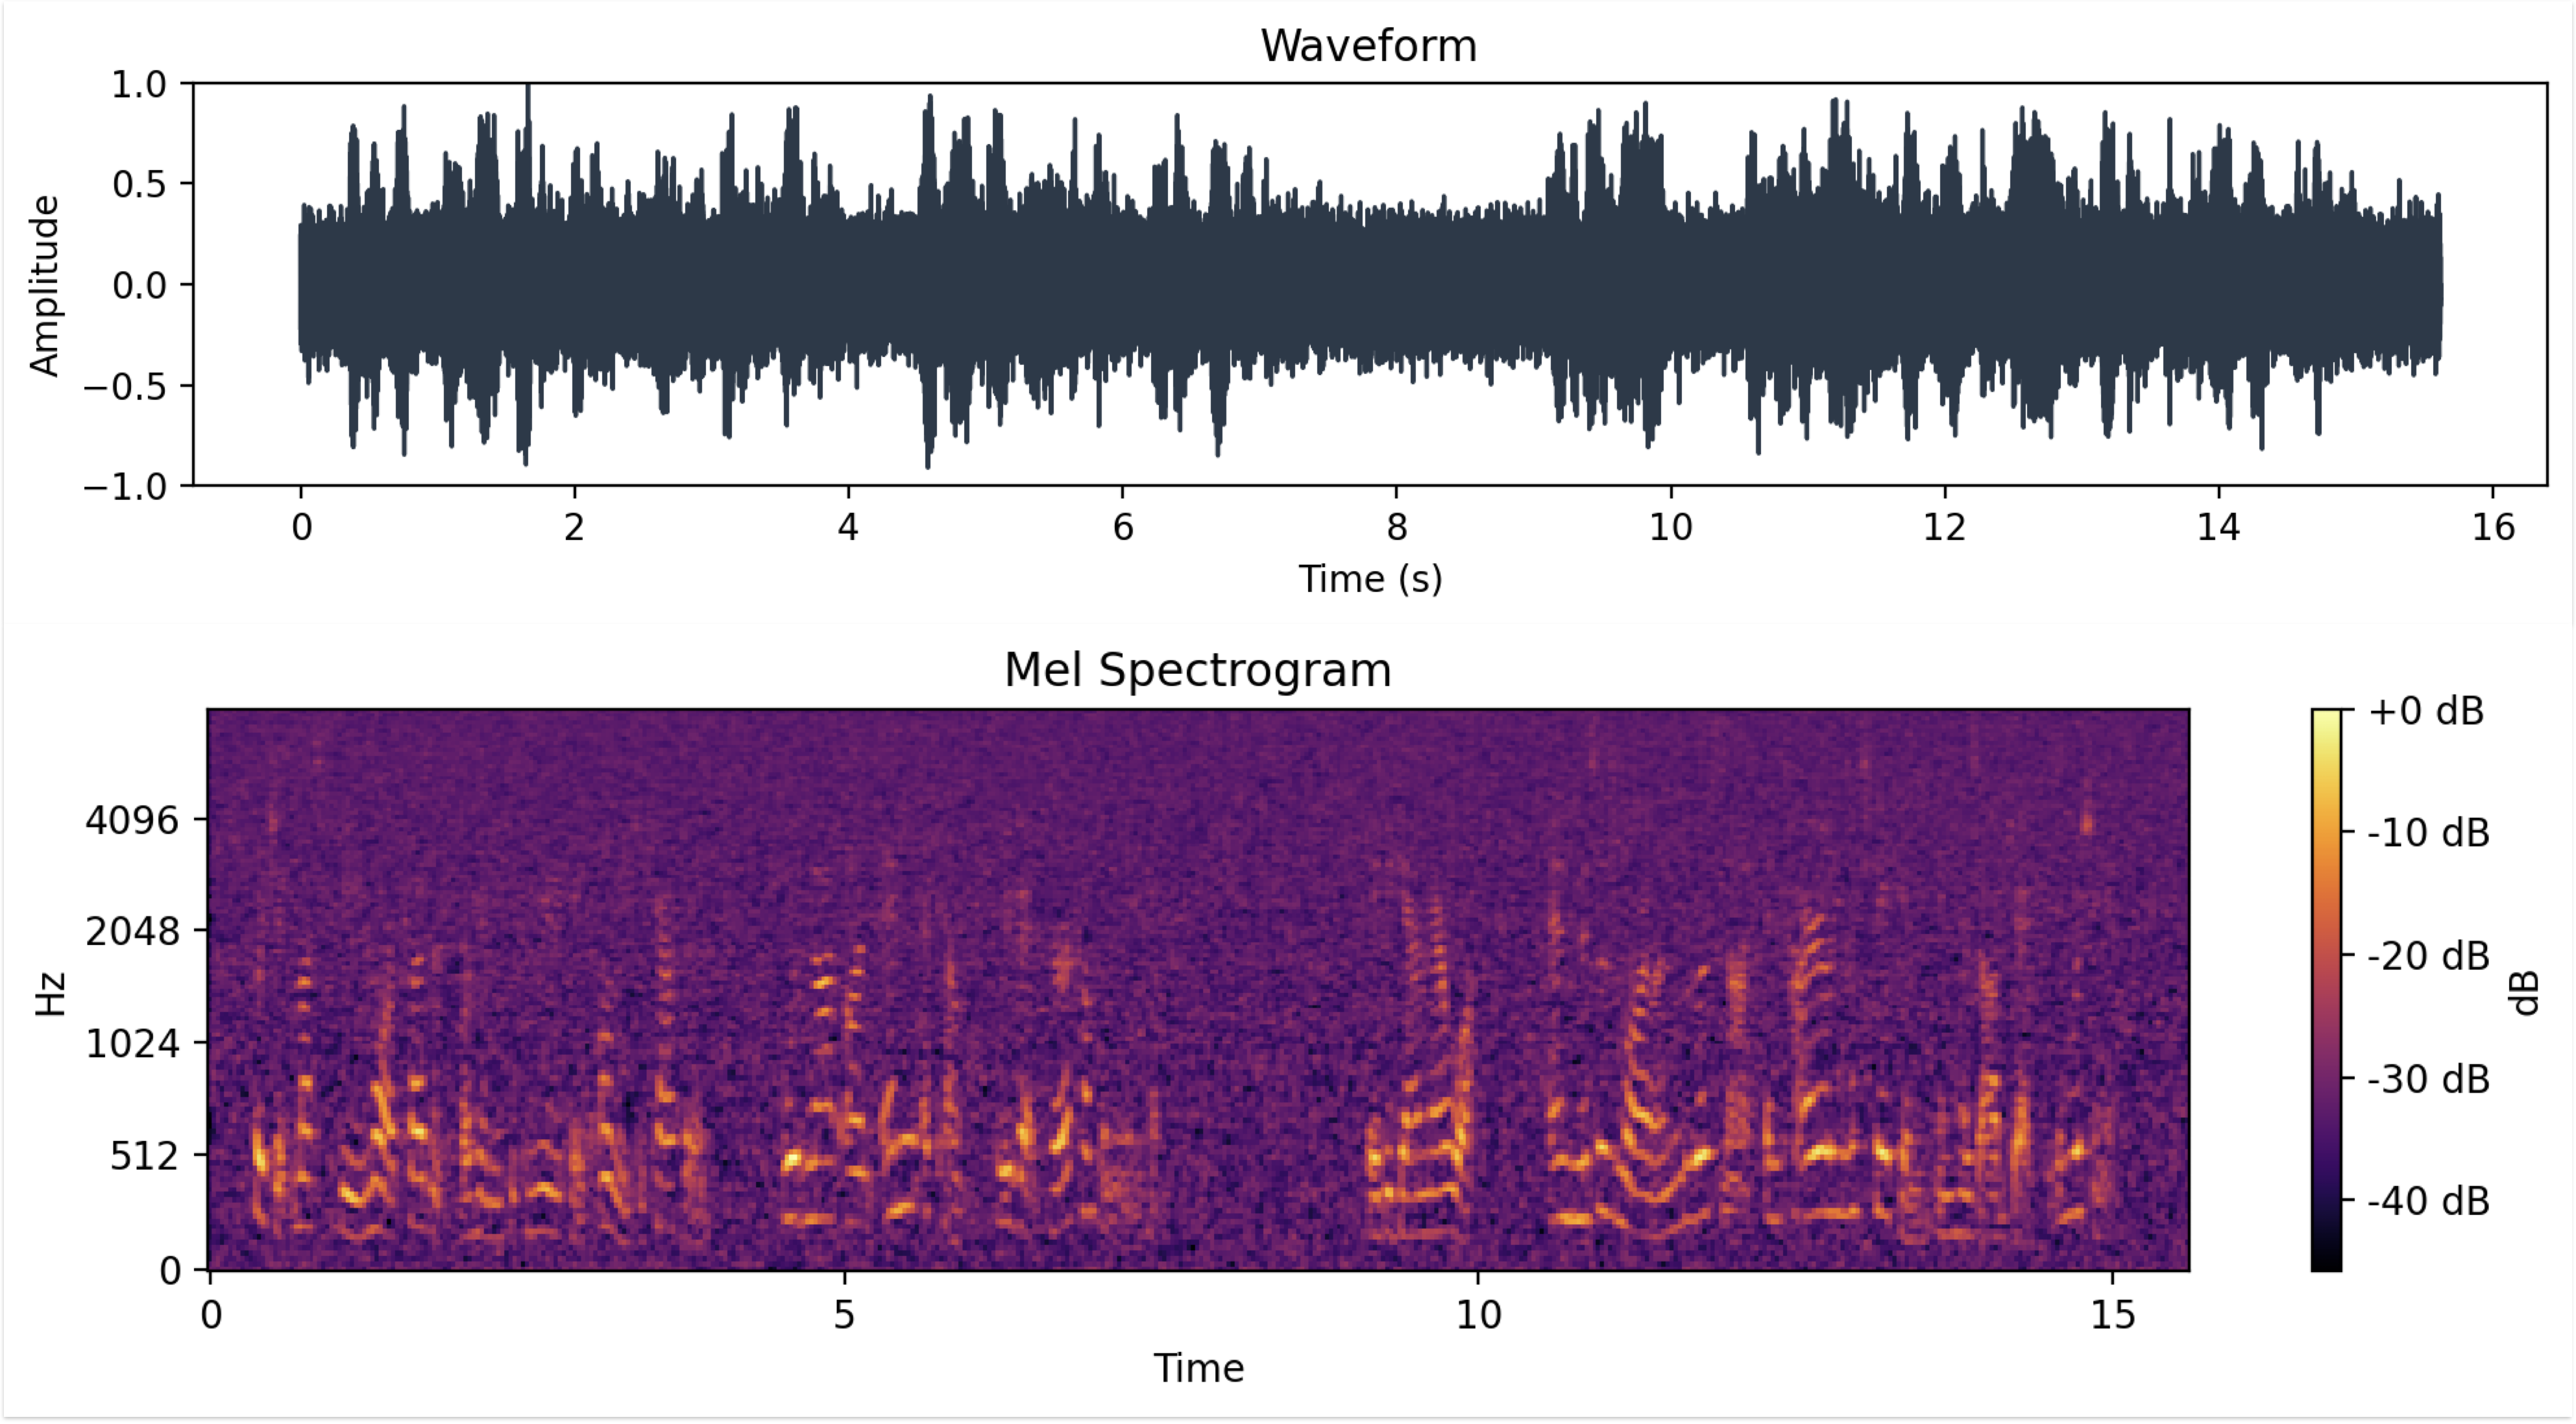
\includegraphics[width=\textwidth]{figures/snr0_o.png}
             \caption{Noisy Speech Signal}
             \label{fig:y equals x}
         \end{subfigure}
         \hfill
         \begin{subfigure}[b]{0.3\textwidth}
             \centering
             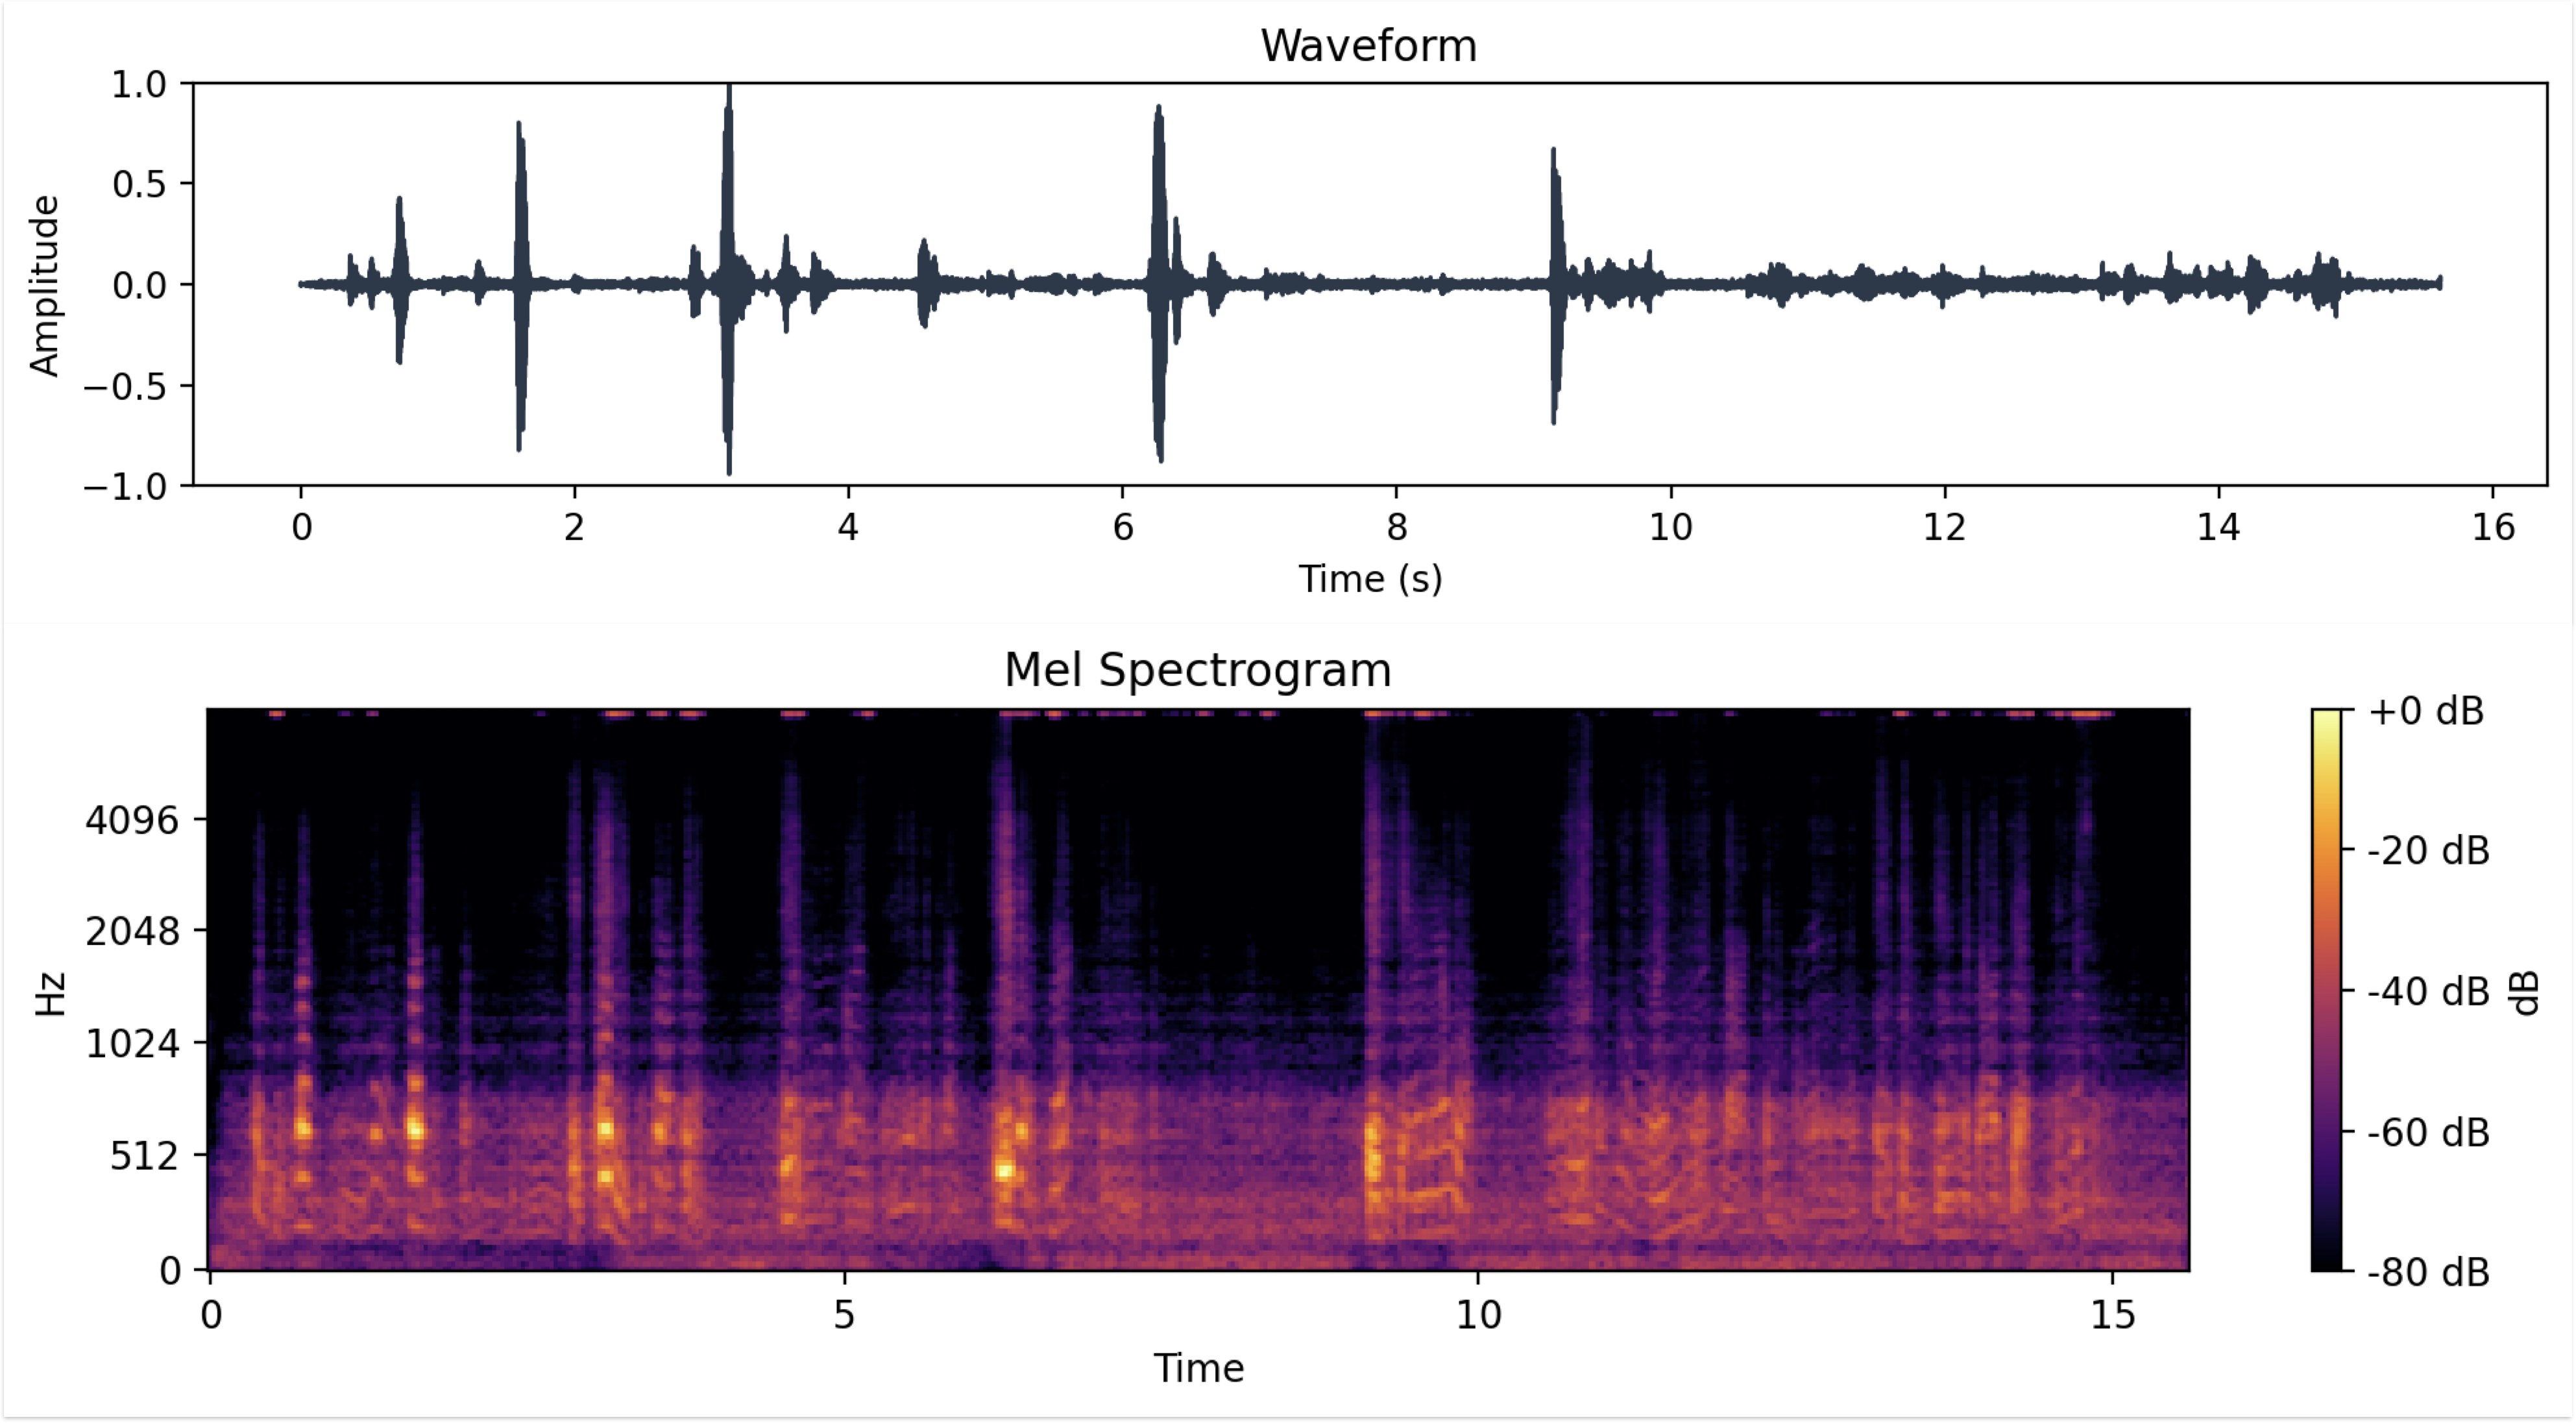
\includegraphics[width=\textwidth]{figures/snr0_e.png}
             \caption{MetricGAN Enhancement}
             \label{fig:three sin x}
         \end{subfigure}
         \hfill
         \begin{subfigure}[b]{0.3\textwidth}
             \centering
             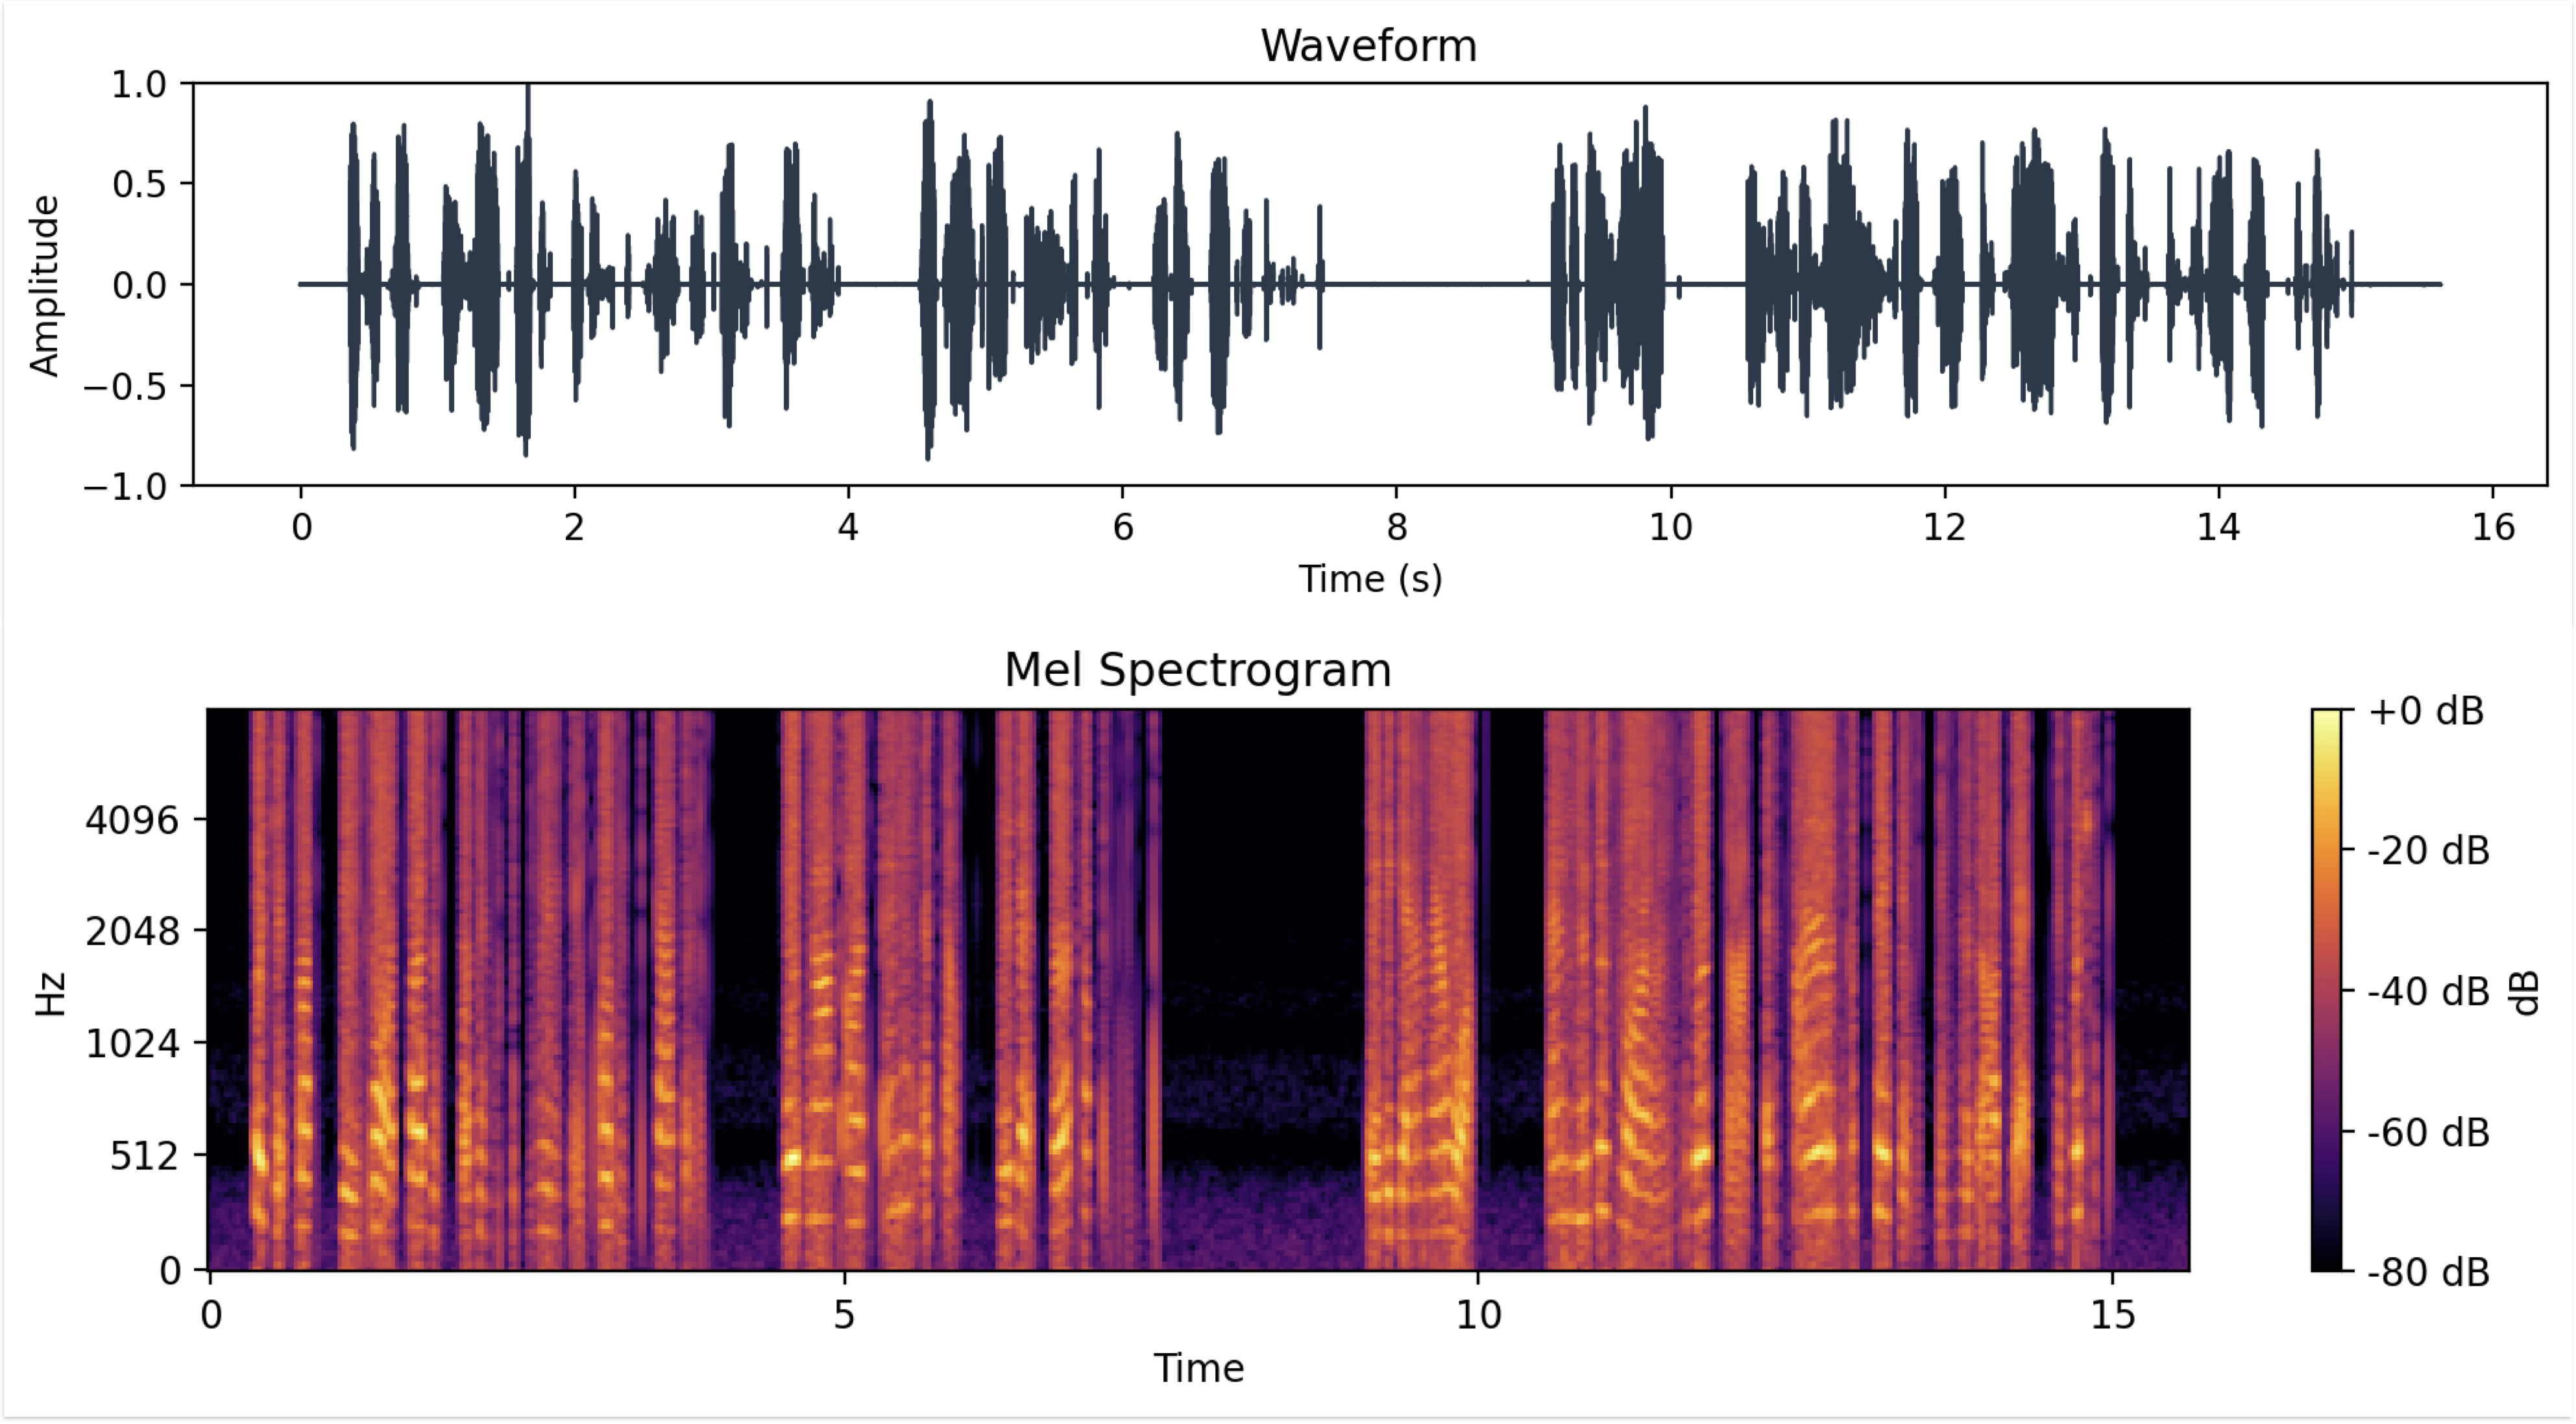
\includegraphics[width=\textwidth]{figures/snr0_w.png}
             \caption{Wiener Filtering}
             \label{fig:five over x}
         \end{subfigure}
            \caption{Speech enhancement results for input signals with an SNR of 0 dB}
            \label{fig:three graphs}
        \vspace{2mm}
    % Finish third block
\end{figure}



\begin{table}[H]
 % Table
    \begin{tabularx}{1\textwidth} { 
      | >{\centering\arraybackslash}X 
      | >{\centering\arraybackslash}X 
      | >{\centering\arraybackslash}X 
      | >{\centering\arraybackslash}X 
      | >{\centering\arraybackslash}X 
      | >{\centering\arraybackslash}X |}
     \hline
      & Noisy & MetricGAN & Wiener & Min-Max & Range\\
     \hline
     PESQ  & 1.06  & 1.12 & 1.05 & 1.05-1.12 & 1.0 - 4.5 \\
     \hline
     STOI  & 0.44  & 0.26 & 0.29 & 0.26-0.44 & 0 - 1 \\
     \hline
     SNR (dB)  & -2.69  & 0.00 & 1.30 & -2.69 - 1.30 & -10 - 30 dB \\
    \hline
    \end{tabularx}
    % Finish table
    \caption{Figure 7.2: In this highly noisy scenario, both MetricGAN and the Wiener filter slightly improve the signal quality compared to the original noisy input. MetricGAN achieves the highest PESQ score (1.12) and matches the input SNR at 0 dB. The Wiener filter slightly surpasses the input with an SNR of 1.30 dB. However, STOI scores are low across all methods, meaning speech remains hard to understand in this very noisy condition. MetricGAN provides a modest advantage in perceptual quality.}
    \label{tab:snr_blocks}
\end{table}

\vspace{2mm}

\begin{figure}[H]
    \centering
         \begin{subfigure}[b]{0.3\textwidth}
             \centering
             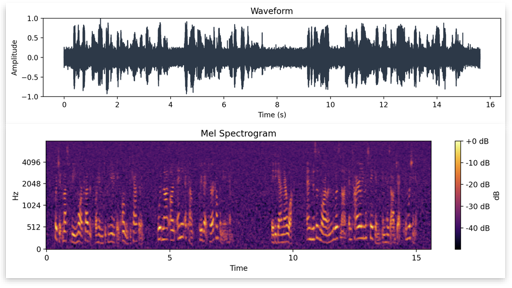
\includegraphics[width=\textwidth]{figures/snr5_o.png}
             \caption{Noisy Speech Signal}
             \label{fig:y equals x}
         \end{subfigure}
         \hfill
         \begin{subfigure}[b]{0.3\textwidth}
             \centering
             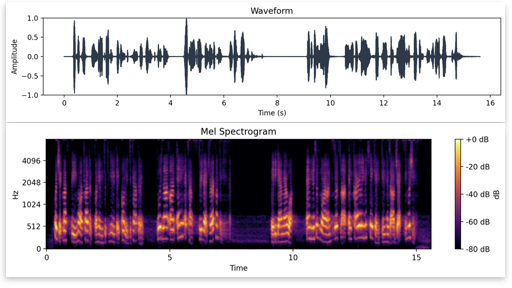
\includegraphics[width=\textwidth]{figures/snr5_e.png}
             \caption{MetricGAN Enhancement}
             \label{fig:three sin x}
         \end{subfigure}
         \hfill
         \begin{subfigure}[b]{0.3\textwidth}
             \centering
             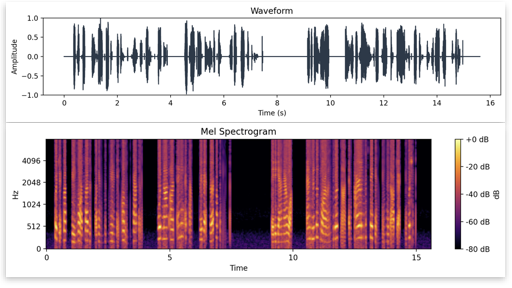
\includegraphics[width=\textwidth]{figures/snr5_w.png}
             \caption{Wiener Filtering}
             \label{fig:five over x}
         \end{subfigure}
            \caption{Speech enhancement results for input signals with an SNR of 5 dB}
            \label{fig:three graphs}
        
    % Finish third block
\end{figure}

\begin{table}[H]
 % Table
    \begin{tabularx}{1\textwidth} { 
      | >{\centering\arraybackslash}X 
      | >{\centering\arraybackslash}X 
      | >{\centering\arraybackslash}X 
      | >{\centering\arraybackslash}X 
      | >{\centering\arraybackslash}X 
      | >{\centering\arraybackslash}X |}
     \hline
      & Noisy & MetricGAN & Wiener & Min-Max & Range\\
     \hline
     PESQ      & 1.12  & 1.91 & 1.07  & 1.07 - 1.91 & 0.5 - 4.5 \\
    \hline
    STOI      & 0.56  & 0.54 & 0.36  & 0.36 - 0.56 & 0 - 1 \\
    \hline
    SNR (dB)  & -0.16 & 2.39 & 1.96  & -0.16 - 2.39 & -10 - 30 dB \\
    \hline
    \end{tabularx}
    % Finish table
    \caption{Figure 7.3: MetricGAN significantly enhances speech quality, raising the PESQ score from 1.12 (noisy input) to 1.91 and improving SNR from –0.16 dB to 2.39 dB. The Wiener filter also improves quality, though less effectively. STOI scores remain similar for both MetricGAN and the noisy input, suggesting limited gains in intelligibility. MetricGAN clearly outperforms the Wiener filter in terms of overall signal clarity and perceptual quality.}
    \label{tab:snr_blocks}
\end{table}

\vspace{2mm}

\begin{figure}[H]
    \centering
         \begin{subfigure}[b]{0.3\textwidth}
             \centering
             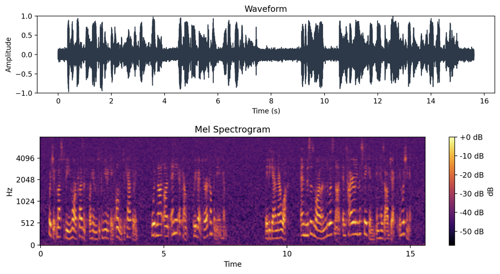
\includegraphics[width=\textwidth]{figures/snr10_o.png}
             \caption{Noisy Speech Signal}
             \label{fig:y equals x}
         \end{subfigure}
         \hfill
         \begin{subfigure}[b]{0.3\textwidth}
             \centering
             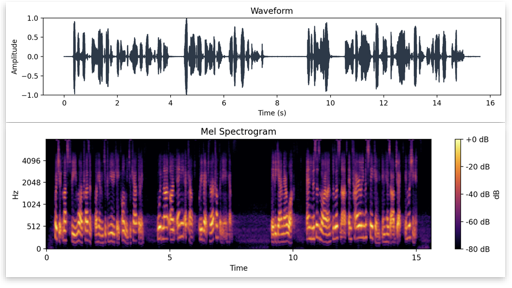
\includegraphics[width=\textwidth]{figures/snr10_e.png}
             \caption{MetricGAN Enhancement}
             \label{fig:three sin x}
         \end{subfigure}
         \hfill
         \begin{subfigure}[b]{0.3\textwidth}
             \centering
             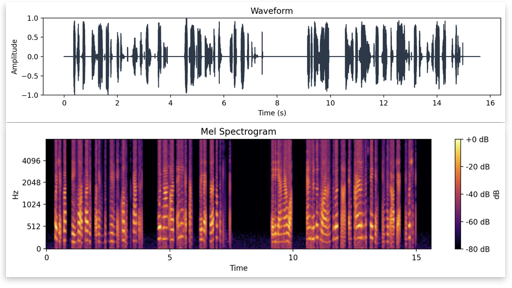
\includegraphics[width=\textwidth]{figures/snr10_w.png}
             \caption{Wiener Filtering}
             \label{fig:five over x}
         \end{subfigure}
            \caption{Speech enhancement results for input signals with an SNR of 10 dB}
            \label{fig:three graphs}
    % Finish third block
\end{figure}

\begin{table}[H]
 % Table
    \begin{tabularx}{1\textwidth} { 
      | >{\centering\arraybackslash}X 
      | >{\centering\arraybackslash}X 
      | >{\centering\arraybackslash}X 
      | >{\centering\arraybackslash}X 
      | >{\centering\arraybackslash}X 
      | >{\centering\arraybackslash}X |}
    \hline
          & Noisy & MetricGAN & Wiener & Min-Max & Range\\
         \hline
        PESQ      & 1.25  & 2.39 & 1.08  & 1.08 - 2.39 & 0.5 - 4.5 \\
        \hline
        STOI      & 0.67  & 0.67 & 0.41  & 0.41 - 0.67 & 0 - 1 \\
        \hline
        SNR (dB)  & 2.90  & 3.81 & 2.62  & 2.62 - 3.81 & -10 - 30 dB \\
        \hline
    \end{tabularx}
    % Finish table
    \caption{Figure 7.4: At 10 dB, both enhancement methods improve the speech signal compared to the noisy input. MetricGAN leads with the highest increase in PESQ (2.39) and SNR (3.81 dB). STOI remains equally good for both MetricGAN and the noisy input (0.67), reflecting good intelligibility, but MetricGAN offers clearer overall audio quality. The Wiener filter improves SNR but falls behind MetricGAN in both PESQ and STOI scores. This highlights MetricGAN's effectiveness at moderate noise levels.}
    \label{tab:snr_blocks}
\end{table}

\vspace{2mm}

\begin{figure}[H]
    \centering
         \begin{subfigure}[b]{0.3\textwidth}
             \centering
             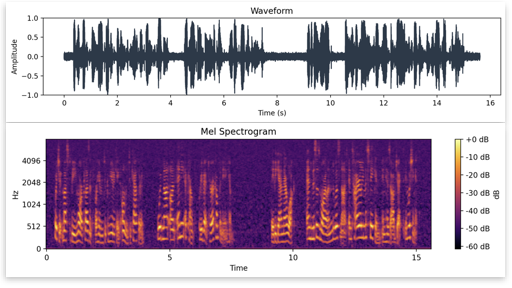
\includegraphics[width=\textwidth]{figures/snr15_o.png}
             \caption{Noisy Speech Signal}
             \label{fig:y equals x}
         \end{subfigure}
         \hfill
         \begin{subfigure}[b]{0.3\textwidth}
             \centering
             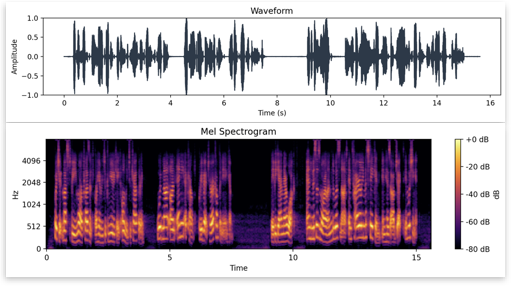
\includegraphics[width=\textwidth]{figures/snr15_e.png}
             \caption{MetricGAN Enhancement}
             \label{fig:three sin x}
         \end{subfigure}
         \hfill
         \begin{subfigure}[b]{0.3\textwidth}
             \centering
             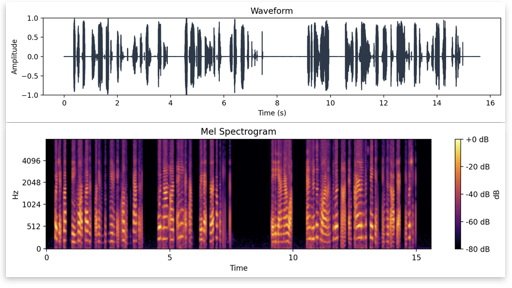
\includegraphics[width=\textwidth]{figures/snr15_w.png}
             \caption{Wiener Filtering}
             \label{fig:five over x}
         \end{subfigure}
            \caption{Speech enhancement results for input signals with an SNR of 15 dB}
            \label{fig:three graphs}
        \vspace{2mm}
    % Finish third block
\end{figure}

\begin{table}[H]
 % Table
    \begin{tabularx}{1\textwidth} { 
      | >{\centering\arraybackslash}X 
      | >{\centering\arraybackslash}X 
      | >{\centering\arraybackslash}X 
      | >{\centering\arraybackslash}X 
      | >{\centering\arraybackslash}X 
      | >{\centering\arraybackslash}X |}
     \hline
      & Noisy & MetricGAN & Wiener & Min-Max & Range\\
     \hline
     PESQ      & 1.51  & 2.79 & 1.09  & 1.09 - 2.79 & 0.5 - 4.5 \\
    \hline
    STOI      & 0.75  & 0.74 & 0.43  & 0.43 - 0.75 & 0 - 1 \\
    \hline
    SNR (dB)  & 6.56  & 5.17 & 3.01  & 3.01 - 6.56 & -10 - 30 dB \\
    \hline
    \end{tabularx}
    % Finish table
    \caption{Figure 7.5: With cleaner inputs, MetricGAN improves the perceptual quality, achieving a PESQ of 2.79 and maintaining high STOI (0.74), slightly better than the noisy input and Wiener filter. Both methods produce clear speech outputs, but MetricGAN consistently excels in perceptual quality and intelligibility, clearly visible in the spectrogram improvements.}
    \label{tab:snr_blocks}
\end{table}

\vspace{2mm}


\begin{figure}[H]
    \centering
         \begin{subfigure}[b]{0.3\textwidth}
             \centering
             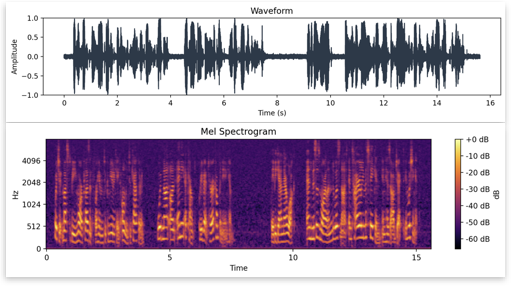
\includegraphics[width=\textwidth]{figures/snr20_o.png}
             \caption{Noisy Speech Signal}
             \label{fig:y equals x}
         \end{subfigure}
         \hfill
         \begin{subfigure}[b]{0.3\textwidth}
             \centering
             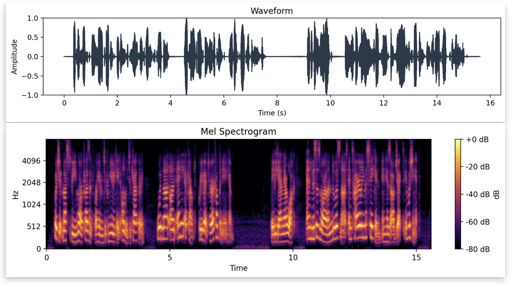
\includegraphics[width=\textwidth]{figures/snr20_e.png}
             \caption{MetricGAN Enhancement}
             \label{fig:three sin x}
         \end{subfigure}
         \hfill
         \begin{subfigure}[b]{0.3\textwidth}
             \centering
             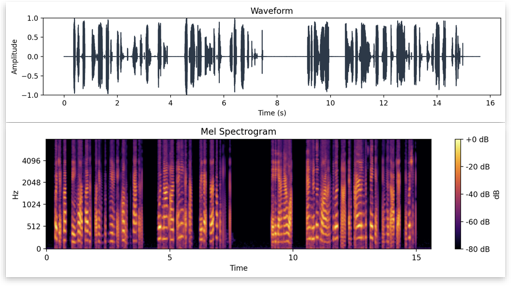
\includegraphics[width=\textwidth]{figures/snr20_w.png}
             \caption{Wiener Filtering}
             \label{fig:five over x}
         \end{subfigure}
            \caption{Speech enhancement results for input signals with an SNR of 20 dB}
            \label{fig:three graphs}
    % Finish third block
\end{figure}

\begin{table}[H]
 % Table
    \begin{tabularx}{1\textwidth} { 
      | >{\centering\arraybackslash}X 
      | >{\centering\arraybackslash}X 
      | >{\centering\arraybackslash}X 
      | >{\centering\arraybackslash}X 
      | >{\centering\arraybackslash}X 
      | >{\centering\arraybackslash}X |}
     \hline
      & Noisy & MetricGAN & Wiener & Min-Max & Range\\
     \hline
     PESQ      & 1.92  & 2.92 & 1.09  & 1.09 - 2.92 & 0.5 - 4.5 \\
    \hline
    STOI      & 0.83  & 0.79 & 0.47  & 0.47 - 0.83 & 0 - 1 \\
    \hline
    SNR (dB)  & 11.16 & 6.35 & 3.12  & 3.12 - 11.16 & -10 - 30 dB \\
    \hline
    \end{tabularx}
    % Finish table
    \caption{Figure 7.6: At 20 dB, the input signal is already quite clean. MetricGAN achieves the highest PESQ score (2.92), but the original noisy input retains slightly higher STOI (0.83) and SNR (11.16 dB). Enhancement improvements are smaller because the audio quality is already high. The Wiener filter only slightly improves or even reduces perceptual quality (PESQ), possibly due to over-smoothing effects. MetricGAN remains a robust and effective choice across various conditions.}
    \label{tab:snr_blocks}
\end{table}


The results show that MetricGAN improves speech quality more effectively than the classical Wiener filter in all tested noise conditions. MetricGAN raises both the clarity and quality of speech, as seen in higher PESQ and SNR scores, and keeps intelligibility high even when noise is strong. These benefits are especially clear when the original audio is very noisy. As the input becomes cleaner, the advantage of using enhancement methods decreases, but MetricGAN still produces consistently good results. Overall, MetricGAN proves to be a reliable and effective method for speech enhancement in a variety of real-world noise scenarios.


\newpage

\chapter{Conclusion}

This thesis explored the use of MetricGAN, a deep learning approach, for speech enhancement under various noise conditions. Experiments were conducted at different noise levels (0 dB, 5 dB, 10 dB, 15 dB, and 20 dB) and compared MetricGAN's performance with a traditional Wiener filter.

The results demonstrated that MetricGAN consistently outperformed the Wiener filter, especially in improving perceptual speech quality (PESQ scores). MetricGAN showed significant advantages in moderately noisy conditions, clearly enhancing both audio clarity and quality. However, in extremely noisy scenarios (0 dB), intelligibility improvements remained limited for all methods.

Overall, MetricGAN proved to be a robust and effective solution for enhancing speech signals, particularly where classical methods like the Wiener filter fall short. Future research could further optimize MetricGAN for extremely challenging conditions and investigate integrating visual information or other complementary techniques to enhance intelligibility even further.


\newpage

\appendix
\chapter{Code Listings}

The source of the code

\href{https://github.com/bakievelbek/project-thesis}{Project GitHub Repository}

\href{https://github.com/speechbrain/speechbrain}{Speechbrain GitHub Repository}


\section{Source code of MetricGAN Model} \label{appendix:metricgan}
\begin{lstlisting}[language=Python, caption={MetricGAN Model}]
import torch
from torch import nn
from torch.nn.utils import spectral_norm

import speechbrain as sb

def xavier_init_layer(
    in_size, out_size=None, spec_norm=True, layer_type=nn.Linear, **kwargs
):
    if out_size is None:
        out_size = in_size

    layer = layer_type(in_size, out_size, **kwargs)
    if spec_norm:
        layer = spectral_norm(layer)

    # Perform initialization
    nn.init.xavier_uniform_(layer.weight, gain=1.0)
    nn.init.zeros_(layer.bias)

    return layer

def shifted_sigmoid(x):
    return 1.2 / (1 + torch.exp(-(1 / 1.6) * x))

class Learnable_sigmoid(nn.Module):

    def __init__(self, in_features=257):
        super().__init__()
        self.slope = nn.Parameter(torch.ones(in_features))
        self.slope.requiresGrad = True


    def forward(self, x):
        return 1.2 * torch.sigmoid(self.slope * x)

class EnhancementGenerator(nn.Module):
    def __init__(
        self,
        input_size=257,
        hidden_size=200,
        num_layers=2,
        dropout=0,
    ):
        super().__init__()
        self.activation = nn.LeakyReLU(negative_slope=0.3)

        self.blstm = sb.nnet.RNN.LSTM(
            input_size=input_size,
            hidden_size=hidden_size,
            num_layers=num_layers,
            dropout=dropout,
            bidirectional=True,
        )
        for name, param in self.blstm.named_parameters():
            if "bias" in name:
                nn.init.zeros_(param)
            elif "weight_ih" in name:
                nn.init.xavier_uniform_(param)
            elif "weight_hh" in name:
                nn.init.orthogonal_(param)

        self.linear1 = xavier_init_layer(400, 300, spec_norm=False)
        self.linear2 = xavier_init_layer(300, 257, spec_norm=False)
        self.Learnable_sigmoid = Learnable_sigmoid()
        self.sigmoid = nn.Sigmoid()

    def forward(self, x, lengths):
        out, _ = self.blstm(x, lengths=lengths)
        out = self.linear1(out)
        out = self.activation(out)
        out = self.linear2(out)
        out = self.Learnable_sigmoid(out)

        return out

class MetricDiscriminator(nn.Module):

    def __init__(
        self,
        kernel_size=(5, 5),
        base_channels=15,
        activation=nn.LeakyReLU,
    ):
        super().__init__()

        self.activation = activation(negative_slope=0.3)

        self.BN = nn.BatchNorm2d(num_features=2, momentum=0.01)

        self.conv1 = xavier_init_layer(
            2, base_channels, layer_type=nn.Conv2d, kernel_size=kernel_size
        )
        self.conv2 = xavier_init_layer(
            base_channels, layer_type=nn.Conv2d, kernel_size=kernel_size
        )
        self.conv3 = xavier_init_layer(
            base_channels, layer_type=nn.Conv2d, kernel_size=kernel_size
        )
        self.conv4 = xavier_init_layer(
            base_channels, layer_type=nn.Conv2d, kernel_size=kernel_size
        )

        self.Linear1 = xavier_init_layer(base_channels, out_size=50)
        self.Linear2 = xavier_init_layer(in_size=50, out_size=10)
        self.Linear3 = xavier_init_layer(in_size=10, out_size=1)

    def forward(self, x):
        out = self.BN(x)
        out = self.conv1(out)
        out = self.activation(out)
        out = self.conv2(out)
        out = self.activation(out)
        out = self.conv3(out)
        out = self.activation(out)
        out = self.conv4(out)
        out = self.activation(out)
        out = torch.mean(out, (2, 3))
        out = self.Linear1(out)
        out = self.activation(out)
        out = self.Linear2(out)
        out = self.activation(out)
        out = self.Linear3(out)
        return out
\end{lstlisting}


\section{MetricGAN usage in the code} \label{appendix:metricgan_in_code}
\begin{lstlisting}[language=Python, caption={How the MetricGAN is Used in the System}]
from speechbrain.inference.enhancement import SpectralMaskEnhancement

enhancer = SpectralMaskEnhancement.from_hparams(
    source="speechbrain/metricgan-plus-voicebank",
    savedir="pretrained_models/metricgan-plus-voicebank"
)

\end{lstlisting}
\newpage

\newpage
\begin{thebibliography}{99}

   \bibitem{schroeder}
   Schroeder, M.R. (1999). The Speech Signal. In: \textit{Computer Speech}. Springer Series in Information Sciences, vol 35. Springer, Berlin, Heidelberg.

    \bibitem{luitel2024audio}
    S. Luitel, Y. Liu and M. Anwar, \textit{"Audio Sentiment Analysis with Spectrogram Representations and Transformer Models,"} 2024 Conference on AI, Science, Engineering, and Technology (AIxSET), Laguna Hills, CA, USA, 2024, pp. 149-153, doi: 10.1109/AIxSET62544.2024.00027.

    \bibitem{miotello}
    F. Miotello, M. Pezzoli, L. Comanducci, F. Antonacci and A. Sarti, \textit{"Deep Prior-Based Audio Inpainting Using Multi-Resolution Harmonic Convolutional Neural Networks,"} in IEEE/ACM Transactions on Audio, Speech, and Language Processing, vol. 32, pp. 113-123, 2024, \href{https://ieeexplore.ieee.org/document/10286406}{doi: 10.1109/TASLP.2023.3324556}

    \bibitem{metricgan}
    Szu-Wei Fu, Chien-Feng Liao, Yu Tsao, Shou-De Lin, \textit{"MetricGAN: Generative Adversarial Networks based Black-box Metric Scores Optimization for Speech Enhancement,"} \href{https://arxiv.org/abs/1905.04874}{doi: 10.1109/TASLP.2023.3324556}    
    
    \bibitem{reddy}
    B. S. T. Reddy and V. Jayaraman, \textit{"Application of Wiener Filter Making Signals Orthogonal,"} 2019 International Conference on Vision Towards Emerging Trends in Communication and Networking (ViTECoN), Vellore, India, 2019, pp. 1-6, \href{https://ieeexplore.ieee.org/document/8899689}{doi: 10.1109/ViTECoN.2019.8899689}

    
    \bibitem{loizou}
     Loizou, P.C. (2007). \textit{Speech Enhancement: Theory and Practice (1st ed.). CRC Press.} \href{https://doi.org/10.1201/9781420015836}{doi.org/10.1201/9781420015836}
    

    
    \bibitem{pesq}
    A. W. Rix, J. G. Beerends, M. P. Hollier and A. P. Hekstra, \textit{"Perceptual evaluation of speech quality (PESQ)-a new method for speech quality assessment of telephone networks and codecs,"} 2001 IEEE International Conference on Acoustics, Speech, and Signal Processing. Proceedings (Cat. No.01CH37221), Salt Lake City, UT, USA, 2001, pp. 749-752 vol.2, \href{https://ieeexplore.ieee.org/document/941023}{doi: 10.1109/ICASSP.2001.941023}

    \bibitem{stoi}
    C. H. Taal, R. C. Hendriks, R. Heusdens and J. Jensen, \textit{"A short-time objective intelligibility measure for time-frequency weighted noisy speech,"} 2010 IEEE International Conference on Acoustics, Speech and Signal Processing, Dallas, TX, USA, 2010, pp. 4214-4217, \href{https://ieeexplore.ieee.org/document/5495701}{doi: 10.1109/ICASSP.2010.5495701} 

    
    \bibitem{snr}
    Cadence PCB Solutions, \textit{"What is Signal to Noise Ratio and How to Calculate It,"} Cadence Resources, 2020. [Online]. Available: \href{https://resources.pcb.cadence.com/blog/2020-what-is-signal-to-noise-ratio-and-how-to-calculate-it}{[link]}.
    
    \bibitem{nuha-noise-reduction}
    H. H. Nuha and A. Abo Absa, \textit{"Noise Reduction and Speech Enhancement Using Wiener Filter,"} 2022 International Conference on Data Science and Its Applications (ICoDSA), Bandung, Indonesia, 2022, pp. 177-180, \href{https://ieeexplore.ieee.org/document/9862912}{doi: 10.1109/ICoDSA55874.2022.9862912}

    \bibitem{gmm-manamperi}
     W. Manamperi, P. N. Samarasinghe, T. D. Abhayapala and J. Zhang, \textit{"GMM Based Multi-Stage Wiener Filtering for Low SNR Speech Enhancement,"} 2022 International Workshop on Acoustic Signal Enhancement (IWAENC), Bamberg, Germany, 2022, pp. 1-5, \href{https://ieeexplore.ieee.org/document/9914707}{doi: 10.1109/IWAENC53105.2022.9914707}

    \bibitem{saleem2018dnnlw}
    N. Saleem, M. Irfan, X. Chen and M. Ali, \textit{"Deep Neural Network based Supervised Speech Enhancement in Speech-Babble Noise,"} 2018 IEEE/ACIS 17th International Conference on Computer and Information Science (ICIS), Singapore, 2018, pp. 871-874, \href{https://ieeexplore.ieee.org/document/8466542}{doi: 10.1109/ICIS.2018.8466542}
    
    \bibitem{morrone2021audiovisual}
    G. Morrone, D. Michelsanti, Z. -H. Tan and J. Jensen, \textit{"Audio-Visual Speech Inpainting with Deep Learning,"} ICASSP 2021 - 2021 IEEE International Conference on Acoustics, Speech and Signal Processing (ICASSP), Toronto, ON, Canada, 2021, pp. 6653-6657, \href{https://ieeexplore.ieee.org/document/9413488}{doi: 10.1109/ICASSP39728.2021.9413488}

    \bibitem{schreibman2024frann}
    A. Schreibman, E. Hadad, B. Rubenchik, M. Tzur and E. Tzirkel-Hancock, \textit{"Single-Channel Speech Restoration Using Deep Speech Features Reconstruction,"} 2024 32nd European Signal Processing Conference (EUSIPCO), Lyon, France, 2024, pp. 231-235, \href{https://ieeexplore.ieee.org/document/10715407}{doi: 10.23919/EUSIPCO63174.2024.10715407}

    \bibitem{marafioti}
    A. Marafioti, N. Perraudin, N. Holighaus and P. Majdak, \textit{"A Context Encoder For Audio Inpainting,"} in IEEE/ACM Transactions on Audio, Speech, and Language Processing, vol. 27, no. 12, pp. 2362-2372, Dec. 2019, \href{https://ieeexplore.ieee.org/document/8867915}{doi: 10.1109/TASLP.2019.2947232}
    


    \bibitem{sun2021rnn}
    Z. Sun, Y. Li, H. Jiang and Z. Wang, \textit{"An RNN-based Speech Enhancement Method for a Binaural Hearing Aid System,"} 2019 17th IEEE International New Circuits and Systems Conference (NEWCAS), Munich, Germany, 2019, pp. 1-4, doi: 10.1109/NEWCAS44328.2019.8961268.

%GAN

    \bibitem{hung2024integrating}
    Y. -H. Hung, Y. -C. Chang, S. -C. Lai, W. -H. Juang, M. -H. Sheu and J. -D. Lee, \textit{"Integrating Noise Classification and Speech Enhancement Model for Hearing Aids,"} 2024 21st International SoC Design Conference (ISOCC), Sapporo, Japan, 2024, pp. 368-369, \href{https://ieeexplore.ieee.org/document/10762526}{doi: 10.1109/ISOCC62682.2024.10762526}.

    \bibitem{phan2021selfattention}
    H. Phan et al., \textit{"Self-Attention Generative Adversarial Network for Speech Enhancement,"} ICASSP 2021 - 2021 IEEE International Conference on Acoustics, Speech and Signal Processing (ICASSP), Toronto, ON, Canada, 2021, pp. 7103-7107, \href{https://ieeexplore.ieee.org/document/9414265}{doi: 10.1109/ICASSP39728.2021.9414265}.
    
    \bibitem{xu2022vsegan}
    X. Xu et al., \textit{"VSEGAN: Visual Speech Enhancement Generative Adversarial Network,"} ICASSP 2022 - 2022 IEEE International Conference on Acoustics, Speech and Signal Processing (ICASSP), Singapore, Singapore, 2022, pp. 7308-7311, \href{https://ieeexplore.ieee.org/document/9747187}{doi: 10.1109/ICASSP43922.2022.9747187}.


    \bibitem{liu2020cpgan}
    G. Liu, K. Gong, X. Liang and Z. Chen, \textit{"CP-GAN: Context Pyramid Generative Adversarial Network for Speech Enhancement,"} ICASSP 2020 - 2020 IEEE International Conference on Acoustics, Speech and Signal Processing (ICASSP), Barcelona, Spain, 2020, pp. 6624-6628, \href{https://ieeexplore.ieee.org/document/9054060}{doi: 10.1109/ICASSP40776.2020.9054060}.

    \bibitem{faraji2020afpgan}
    F. Faraji, Y. Attabi, B. Champagne and W. -P. Zhu,\textit{ "On the Use of Audio Fingerprinting Features for Speech Enhancement with Generative Adversarial Network,"} 2020 IEEE Workshop on Signal Processing Systems (SiPS), Coimbra, Portugal, 2020, pp. 1-6, \href{https://ieeexplore.ieee.org/document/9195238}{doi: 10.1109/SiPS50750.2020.9195238}.


    \bibitem{metricgan_model}
    SpeechBrain GitHub repository [Online]. Available: \href{https://github.com/speechbrain/speechbrain/blob/develop/speechbrain/lobes/models/MetricGAN.py}{[link]}.

\end{thebibliography}




\end{document}
